\documentclass{article}
\usepackage[utf8]{inputenc} % Hỗ trợ gõ tiếng Việt với mã UTF-8
\usepackage[T5]{fontenc} % Hỗ trợ font tiếng Việt (cũ, có thể cân nhắc T1)
\usepackage[vietnamese]{babel} % Thiết lập ngôn ngữ tiếng Việt cho tài liệu
\usepackage{indentfirst} % Thêm gói này để thụt đầu dòng đoạn đầu tiên của mục
\usepackage{authblk} % Dùng để định dạng thông tin tác giả và đơn vị
\renewcommand\Authands{ and }
\usepackage{setspace} % Cho phép điều chỉnh khoảng cách dòng (ví dụ: onehalfspacing)
\usepackage[margin=1.25in]{geometry} % Tùy chỉnh lề trang
\usepackage{graphicx} % Để chèn hình ảnh
\graphicspath{{./Figures/}} % Khai báo thư mục chứa hình ảnh
\usepackage{subcaption} % Tạo phụ chú cho các hình ảnh con (subfigures)
\usepackage{amsmath} % Các gói toán học nâng cao của AMS
\usepackage{booktabs} % Tạo bảng đẹp hơn (ví dụ: \toprule, \midrule, \bottomrule)
\usepackage{longtable} % Cho phép bảng kéo dài qua nhiều trang
\usepackage{array} % Cung cấp thêm các tùy chọn cho cột trong bảng
\usepackage{float} % Cải thiện việc đặt các đối tượng nổi (figures, tables) - ví dụ: [H]
\usepackage{placeins} % Cung cấp lệnh \FloatBarrier để ngăn các đối tượng nổi vượt qua điểm đó
\usepackage{pgfplots} % Vẽ đồ thị bằng PGF/TikZ
\usepackage{xcolor} % Cho phép sử dụng màu sắc
\usepackage{tikz} % Ngôn ngữ vẽ đồ họa mạnh mẽ
\usepackage{csquotes} % Xử lý dấu ngoặc kép thông minh, đặc biệt cho biblatex
\usepackage{hyperref} % Tạo siêu liên kết trong tài liệu (ví dụ: cho mục lục, trích dẫn)
\pgfplotsset{compat=1.18} % Đảm bảo tính tương thích cho pgfplots

\usetikzlibrary{shapes.geometric, arrows.meta, positioning, shapes.misc, fit, backgrounds, calc} % Nạp các thư viện TikZ cần thiết cho vẽ sơ đồ
\tikzset{ % Định nghĩa các style chung cho các phần tử trong sơ đồ TikZ
  block/.style={draw, rectangle, rounded corners, align=center, minimum height=2em}, % Khối chữ nhật bo góc
  data/.style={draw, trapezium, trapezium left angle=70, trapezium right angle=110, align=center, minimum height=2em}, % Hình thang (dữ liệu)
  process/.style={draw, rectangle, rounded corners, align=center, minimum height=2em, fill=blue!10}, % Khối xử lý (màu xanh)
  decision/.style={draw, diamond, align=center, minimum height=2em, fill=green!10}, % Khối quyết định (hình thoi, màu xanh lá)
  group/.style={draw, dotted, rounded corners, inner sep=0.5cm, fill=gray!5}, % Khối nhóm (nét đứt, màu xám)
  title/.style={font=\bfseries, above=0.2cm}, % Style cho tiêu đề nhóm
  arrow/.style={thick,->,>=stealth} % Style cho mũi tên
}

\usepackage[style=nejm, % Kiểu trích dẫn NEJM
citestyle=numeric-comp, % Kiểu hiển thị trích dẫn là số, nén lại (ví dụ: [1-3])
sorting=none, % Không sắp xếp tài liệu tham khảo (giữ nguyên thứ tự trong file .bib)
backend=biber]{biblatex} % Sử dụng Biber làm backend cho biblatex
\addbibresource{sample.bib} % Khai báo file .bib chứa tài liệu tham khảo

\author{
    \textbf{Tên môn học:} DỰ ÁN THỰC TẾ\\
    \textbf{Mã học phần:} AER4001\_1 \\
    \textbf{Giảng viên hướng dẫn:} TS. Hà Minh Cường \\
                                   ThS. Hoàng Tích Phúc\\
    \textbf{Thời gian thực hiện:} Học kỳ II năm học 2024-2025\\ 
    \textbf{Sinh viên thực hiện:}Lê Đức Lương \- MSSV: 21021424
}

\affil{Viện Công nghệ Hàng không Vũ trụ, Trường Đại học Công nghệ - Đại học Quốc gia Hà Nội, Hà Nội, Việt Nam} % Đơn vị công tác
\affil[*]{Địa chỉ liên hệ: luongoc130603@gmail.com} % Thông tin liên hệ

\title{Ứng dụng Viễn thám, GIS và Học máy để Xây dựng Bản đồ Dự đoán Nguy cơ Cháy rừng tại tỉnh Gia Lai, Việt Nam} % Tiêu đề của bài báo


\date{} % Bỏ ngày tháng mặc định

\onehalfspacing % Đặt khoảng cách dòng là 1.5
\begin{document} % Bắt đầu nội dung tài liệu

\maketitle % Hiển thị tiêu đề, tác giả, đơn vị

\begin{abstract}
    Cháy rừng là một hiểm họa nghiêm trọng gây thiệt hại lớn về kinh tế, xã hội và môi trường. Nghiên cứu này trình bày kết quả ứng dụng phương pháp tích hợp dữ liệu viễn thám đa nguồn và các mô hình học máy (RF và GTB) trên nền tảng GEE để xây dựng bản đồ phân cấp nguy cơ cháy rừng cho tỉnh Gia Lai. Dữ liệu cho nghiên cứu được thu thập và phân tích trong giai đoạn mùa khô từ tháng 12 năm 2024 đến tháng 4 năm 2025. Kết quả cho thấy mô hình Random Forest đạt hiệu suất tốt hơn với độ chính xác tổng thể 93.05\% và F1-score 0.9317, so với mô hình Gradient Tree Boosting (độ chính xác 83.81\%, F1-score 0.8412). Các yếu tố quan trọng nhất ảnh hưởng đến nguy cơ cháy rừng bao gồm nhiệt độ bề mặt đất, độ cao địa hình, lượng mưa và tốc độ gió. Bản đồ dự đoán nguy cơ cho thấy khoảng 68.3\% diện tích rừng của tỉnh có nguy cơ cháy từ cao đến cực kỳ nguy hiểm, tập trung chủ yếu ở khu vực trung tâm và phía đông của tỉnh. Các kết quả của nghiên cứu cung cấp công cụ hữu ích cho các cơ quan chức năng trong công tác phòng chống cháy rừng. 
\end{abstract} % Kết thúc phần tóm tắt

\section{Giới thiệu} % Bắt đầu Mục 1: Giới thiệu
Cháy rừng là một trong những thiên tai tàn khốc, gây ra những hậu quả nghiêm trọng đối với hệ sinh thái, kinh tế và đời sống con người. Việt Nam, với diện tích rừng đáng kể và điều kiện khí hậu nhiệt đới gió mùa, thường xuyên phải đối mặt với nguy cơ cháy rừng, đặc biệt trong mùa khô. Tỉnh Gia Lai, nằm ở khu vực Tây Nguyên, với đặc điểm thảm thực vật đa dạng và các yếu tố khí hậu khắc nghiệt, là một trong những điểm nóng về cháy rừng. Việc xây dựng các mô hình dự đoán sớm và chính xác nguy cơ cháy rừng đóng vai trò then chốt trong việc chủ động triển khai các biện pháp phòng ngừa, giảm thiệt hại.

Trong những năm gần đây, sự phát triển của công nghệ viễn thám và hệ thống thông tin địa lý (GIS) đã mở ra những hướng tiếp cận mới và hiệu quả cho việc giám sát và mô hình hóa nguy cơ cháy rừng. Dữ liệu từ các vệ tinh như Sentinel-2, MODIS cung cấp thông tin phong phú về trạng thái thảm thực vật, độ ẩm, nhiệt độ bề mặt đất trên phạm vi rộng và có tính cập nhật cao. Đặc biệt, dữ liệu điểm cháy thực tế từ MODIS là nguồn thông tin quan trọng về sự xuất hiện của các vụ cháy, được sử dụng để tạo nhãn cháy cho việc huấn luyện và đánh giá mô hình. Bên cạnh đó, các thuật toán học máy (Machine Learning - ML) như Random Forest (RF) và Gradient Tree Boosting (GTB) đã chứng minh được hiệu quả vượt trội trong việc xử lý các bộ dữ liệu lớn, phức tạp và xây dựng các mô hình dự đoán với độ chính xác cao trong nhiều lĩnh vực, bao gồm cả khoa học môi trường và quản lý thiên tai~\cite{Breiman2001, Friedman2001, ForestFirePredictionML2022}. Nền tảng điện toán đám mây Google Earth Engine (GEE) với khả năng truy cập và xử lý lượng lớn dữ liệu không gian địa lý đã tạo điều kiện thuận lợi cho việc triển khai các nghiên cứu quy mô lớn~\cite{Gorelick2017}.

Nghiên cứu này nhằm mục tiêu ứng dụng phương pháp tích hợp dữ liệu viễn thám đa nguồn và các mô hình học máy (RF và GTB) trên nền tảng GEE để xây dựng bản đồ phân cấp nguy cơ cháy rừng cho tỉnh Gia Lai trong giai đoạn mùa khô dự kiến từ tháng 12 năm 2024 đến tháng 4 năm 2025. Các kết quả của nghiên cứu được kỳ vọng sẽ cung cấp công cụ hữu ích cho các cơ quan chức năng trong công tác phòng chống cháy rừng.

\section{Khu vực nghiên cứu} % Bắt đầu Mục 2: Khu vực nghiên cứu
Nghiên cứu được thực hiện trên toàn bộ địa bàn tỉnh Gia Lai, Việt Nam. Gia Lai có tọa độ địa lý từ 12°58'40" đến 14°37'00" vĩ độ Bắc và từ 107°28'04" đến 108°54'40" kinh độ Đông. Tỉnh có đặc điểm địa hình đa dạng, bao gồm chủ yếu là cao nguyên và núi thấp, nghiêng dần từ Bắc xuống Nam và từ Đông sang Tây. Phía Bắc là cao nguyên Kon Tum, phía Nam là cao nguyên Pleiku tương đối bằng phẳng, trong khi phía Đông và Đông Nam là vùng núi cao thuộc dãy Trường Sơn Nam, xen kẽ là các thung lũng. Thảm thực vật chủ yếu là rừng tự nhiên lá rộng thường xanh, rừng nửa rụng lá và rừng khộp đặc trưng của Tây Nguyên. Bên cạnh đó là các diện tích rừng trồng như thông, keo và các loại cây công nghiệp dài ngày. Khí hậu Gia Lai mang đặc trưng của khí hậu nhiệt đới gió mùa cao nguyên, chia thành hai mùa rõ rệt: mùa mưa và mùa khô. Mùa khô thường kéo dài từ tháng 11 đến tháng 4 năm sau, đây là thời kỳ có nguy cơ cháy rừng cao nhất.

\begin{figure}[H] % Môi trường figure để chèn hình ảnh, [H] ép hình ảnh xuất hiện tại vị trí khai báo
\centering % Căn giữa hình ảnh
\begin{tikzpicture} % Bắt đầu môi trường vẽ TikZ
\begin{axis}[ % Bắt đầu môi trường trục tọa độ của pgfplots
    ybar, % Loại biểu đồ cột đứng
    xlabel={Tháng}, % Nhãn trục x
    ylabel={Lượng mưa trung bình (mm)}, % Nhãn trục y
    xtick=data, % Vị trí các dấu tick trên trục x dựa vào dữ liệu
    xticklabels={5/24, 6/24, 7/24, 8/24, 9/24, 10/24, 11/24, 12/24, 1/25, 2/25, 3/25, 4/25}, % Nhãn cho các dấu tick trên trục x
    xticklabel style={rotate=45, anchor=east, font=\small}, % Định dạng nhãn trục x (xoay, vị trí, cỡ chữ)
    ymin=0, % Giá trị nhỏ nhất của trục y
    width=1\textwidth, % Chiều rộng của biểu đồ bằng chiều rộng của văn bản
    height=7cm, % Chiều cao của biểu đồ
    bar width=7pt, % Độ rộng của các cột
    enlarge x limits=0.05, % Mở rộng giới hạn trục x một chút
    ymajorgrids=true, % Hiển thị lưới chính trên trục y
    grid style=dashed, % Kiểu lưới là nét đứt
]
\addplot coordinates { % Thêm dữ liệu cho biểu đồ
    (1, 134)
    (2, 117)
    (3, 129)
    (4, 138)
    (5, 200)
    (6, 172)
    (7, 121)
    (8, 46)
    (9, 13)
    (10, 6)
    (11, 21)
    (12, 63)
};
\end{axis} % Kết thúc môi trường trục tọa độ
\end{tikzpicture} % Kết thúc môi trường vẽ TikZ
\caption{Biểu đồ lượng mưa trung bình hàng tháng tại Gia Lai (giai đoạn 5/2024 - 4/2025).} % Chú thích cho hình ảnh
\label{fig:luong_mua_gia_lai} % Nhãn để tham chiếu đến hình ảnh này
\end{figure}
\FloatBarrier % Ngăn không cho các đối tượng nổi (float) vượt qua điểm này

\begin{figure}[H]
\centering
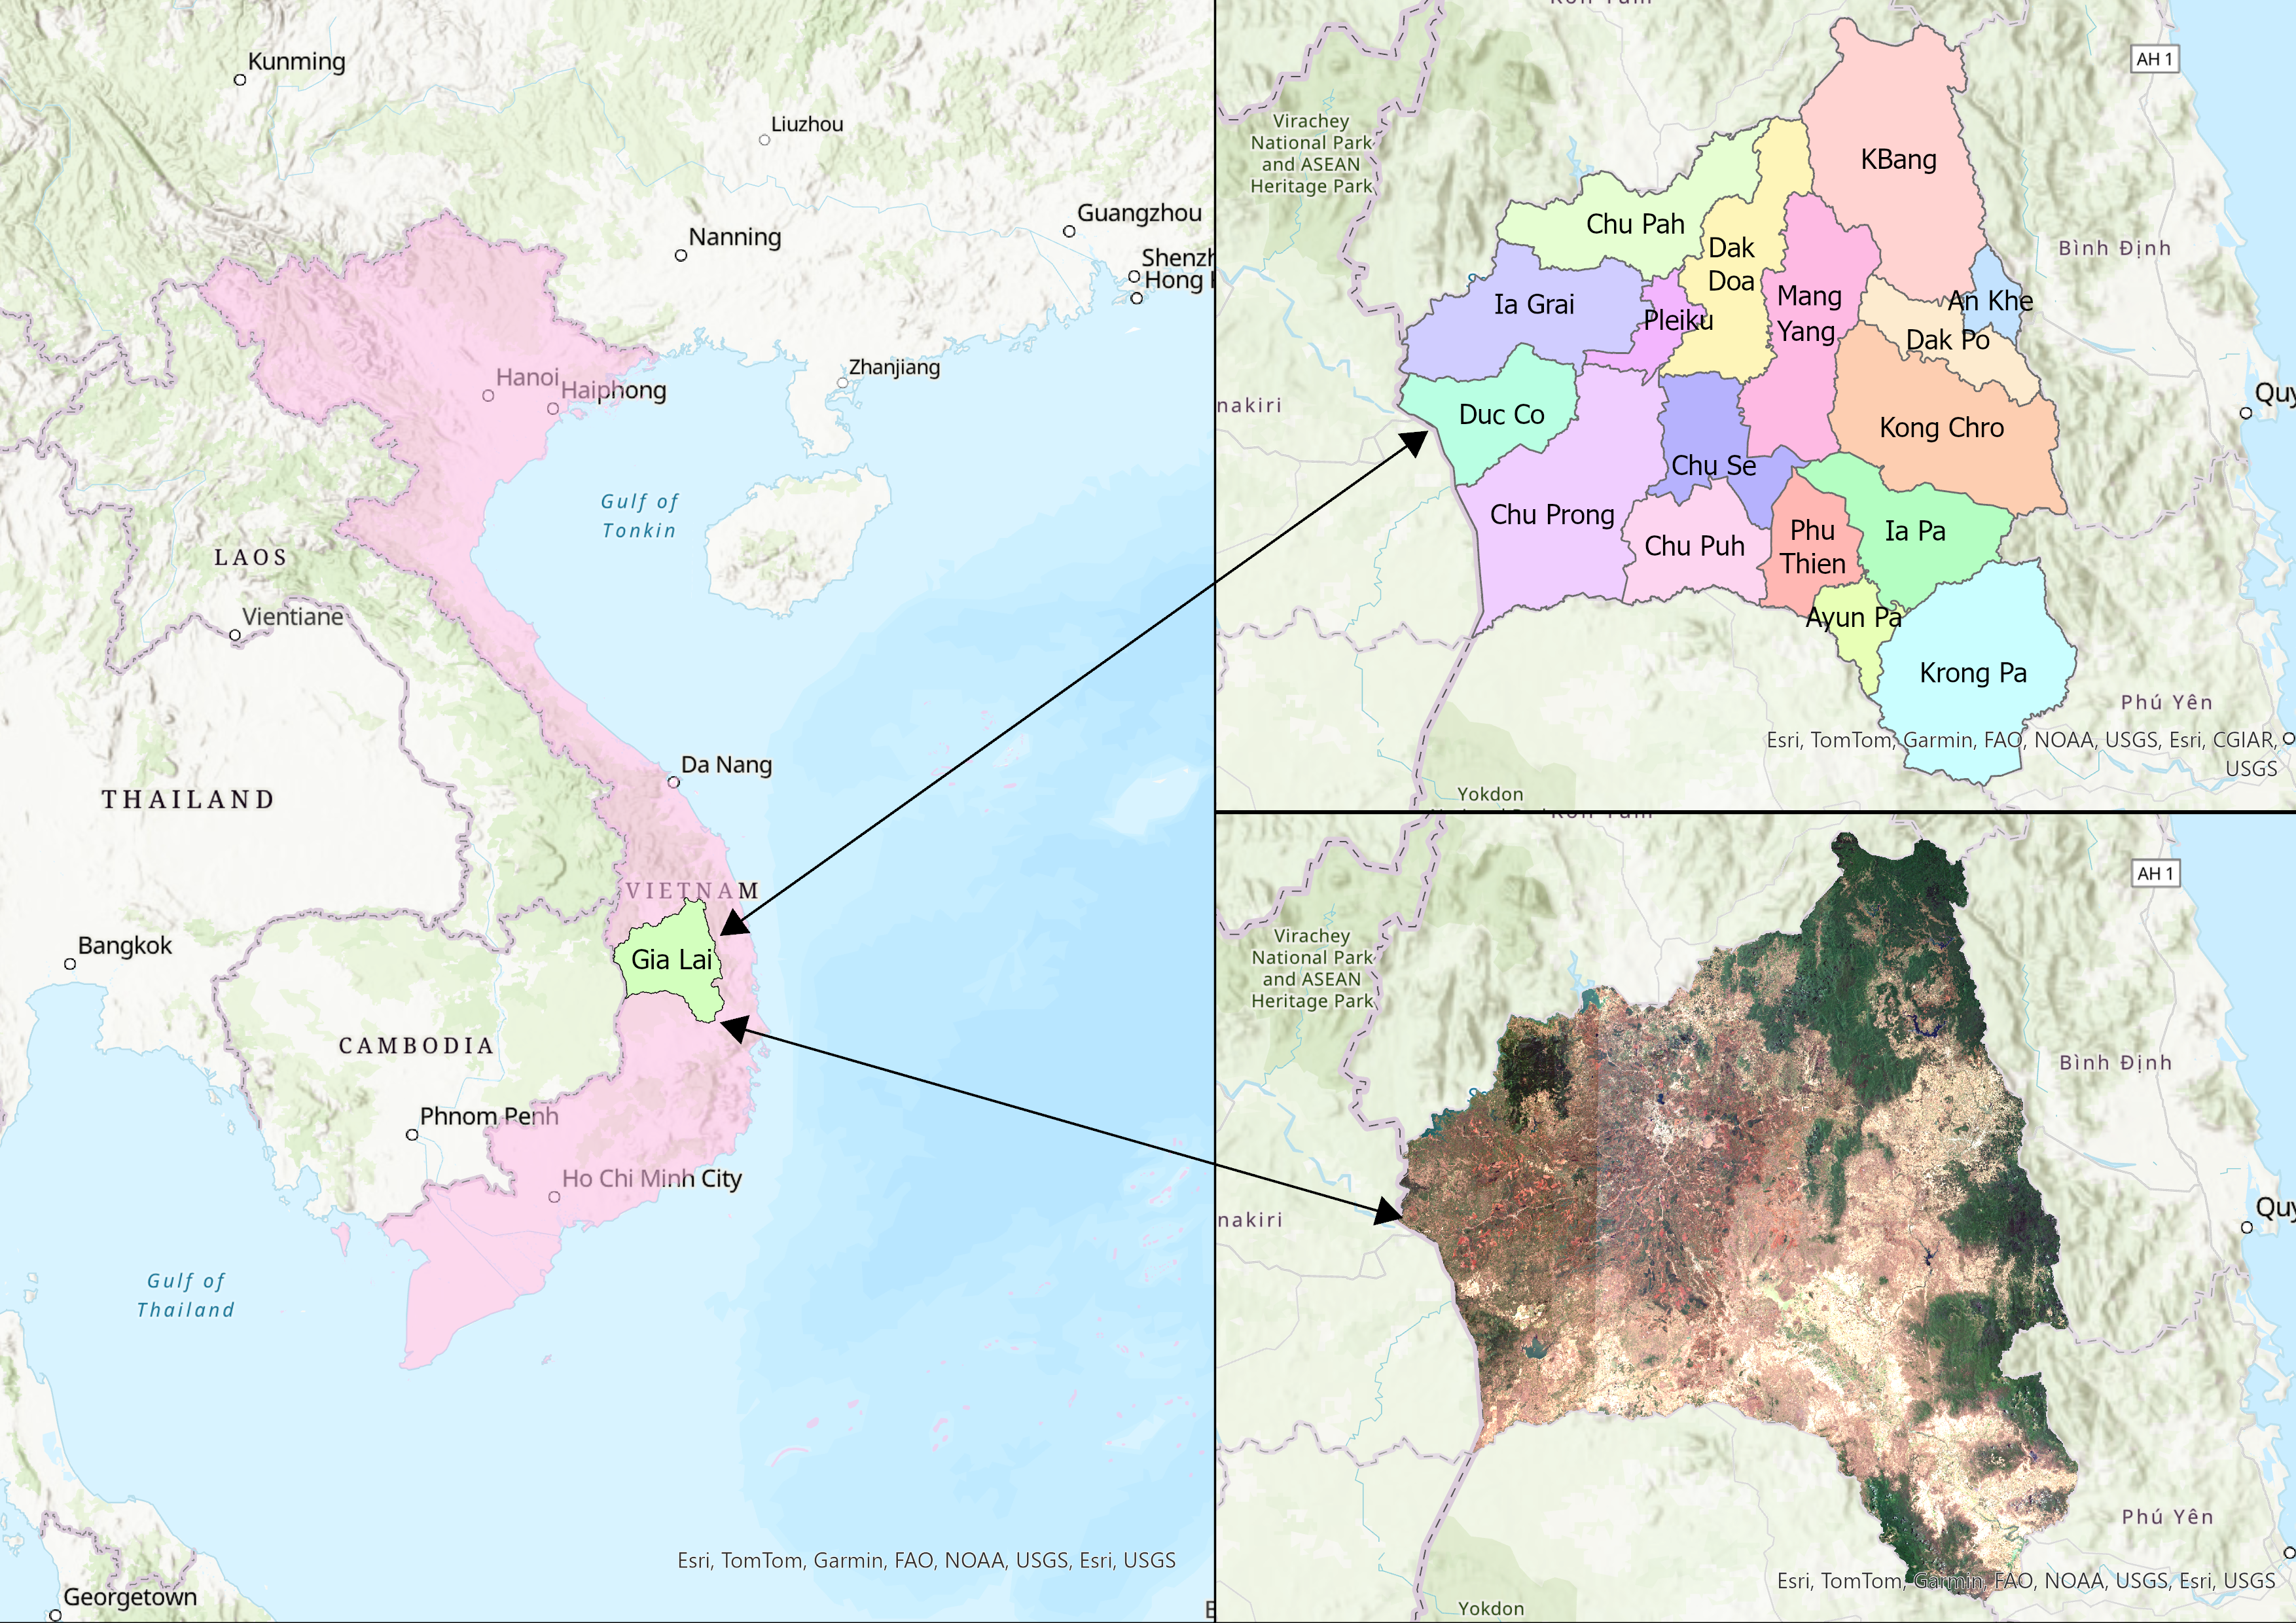
\includegraphics[width=1\textwidth]{Ban_do.png} % Chèn hình ảnh Ban_do.png, chiều rộng bằng chiều rộng văn bản
\caption{Bản đồ vị trí khu vực nghiên cứu tỉnh Gia Lai.}
\label{fig:vi_tri_khu_vuc_nghien_cuu}
\end{figure}

\section{Dữ liệu và Phương pháp} % Bắt đầu Mục 3: Dữ liệu và Phương pháp
Phần này mô tả các bộ dữ liệu được sử dụng và quy trình phương pháp luận được áp dụng trong nghiên cứu.

\subsection{Thu thập và Tiền xử lý Dữ liệu} % Mục con 3.1: Thu thập và Tiền xử lý Dữ liệu
Các bộ dữ liệu viễn thám và phụ trợ sau đây đã được sử dụng trong nghiên cứu (Bảng~\ref{tab:tong_hop_du_lieu}). Các lớp dữ liệu raster đầu vào có độ phân giải không gian khác nhau; ví dụ, dữ liệu Sentinel-2 có các kênh ở 10m, 20m và 60m, trong khi dữ liệu Nhiệt độ Bề mặt Đất (LST) từ MODIS và chỉ số TCI được xử lý ở độ phân giải 1km. Dữ liệu Mô hình số độ cao (DEM) SRTM có độ phân giải 30m. Dữ liệu điểm cháy MODIS (\texttt{FireMask}) được sử dụng để tạo nhãn cháy cho mô hình được xử lý ở độ phân giải 500m.
\begin{itemize} % Môi trường danh sách (gạch đầu dòng)
    \item Ảnh vệ tinh Sentinel-2 MSI (\texttt{COPERNICUS/S2\_SR})~\cite{Drusch2012} được sử dụng để tính toán các chỉ số thực vật và độ ẩm. Các ảnh trong khoảng thời gian từ \texttt{startDate} ("2024-12-01") đến \texttt{endDate} ("2025-04-30") có độ che phủ mây dưới 10\% được lựa chọn. Mây được che phủ dựa trên kênh xác suất mây (\texttt{MSK\_CLDPRB} < 30). Ảnh tổng hợp trung vị (median composite) được tạo ra và cắt theo ranh giới tỉnh Gia Lai.
    \item Dữ liệu Nhiệt độ Bề mặt Đất (LST) ban ngày từ MODIS (\texttt{MODIS/061/MOD11A2})~\cite{Wan2014} được sử dụng để phản ánh điều kiện nhiệt.
    \item Dữ liệu Mô hình số độ cao (DEM) từ SRTM (\texttt{USGS/SRTMGL1\_003})~\cite{Farr2007} được sử dụng để tính toán các yếu tố địa hình.
    \item Dữ liệu Lượng mưa hàng ngày từ CHIRPS (\texttt{UCSB-CHG/CHIRPS/DAILY})~\cite{Funk2015}.
    \item Dữ liệu Gió hàng ngày từ ERA5 Land (\texttt{ECMWF/ERA5\_LAND/DAILY\_AGGR})~\cite{MunozSabater2021}.
    \item Dữ liệu điểm cháy lịch sử từ MODIS (\texttt{MODIS/061/MOD14A1})~\cite{Justice2002} được sử dụng để tạo nhãn cháy cho việc huấn luyện mô hình. Các pixel có giá trị \texttt{FireMask} > 6 được coi là có cháy.
\end{itemize}

\begin{table}[H]
\centering
\caption{Tổng hợp các bộ dữ liệu đã sử dụng.}
\label{tab:tong_hop_du_lieu}
\begin{tabular}{p{5cm}p{5cm}p{3cm}} % Định dạng cột cho bảng: p{width} - cột có chiều rộng cố định, nội dung canh đều
\toprule % Đường kẻ ngang trên cùng của bảng (từ gói booktabs)
\textbf{Tên dữ liệu} & \textbf{Nguồn gốc (Mã sản phẩm GEE)} & \textbf{Độ phân giải} \\
\midrule % Đường kẻ ngang giữa tiêu đề và nội dung (từ gói booktabs)
Ảnh Sentinel-2 MSI & \texttt{COPERNICUS/S2\_SR} & 10m, 20m, 60m \\
Nhiệt độ bề mặt đất MODIS & \texttt{MODIS/061/MOD11A2} & 1km \\
Mô hình số độ cao SRTM & \texttt{USGS/SRTMGL1\_003} & 30m \\
Lượng mưa CHIRPS & \texttt{UCSB-CHG/CHIRPS} & $\sim$5.5km \\
Gió ERA5 Land & \texttt{ECMWF/ERA5\_LAND} & $\sim$9km \\
Điểm cháy MODIS & \texttt{MODIS/061/MOD14A1} & 500m \\
\bottomrule % Đường kẻ ngang dưới cùng của bảng (từ gói booktabs)
\end{tabular}
\end{table}

\begin{figure}[H]
\centering
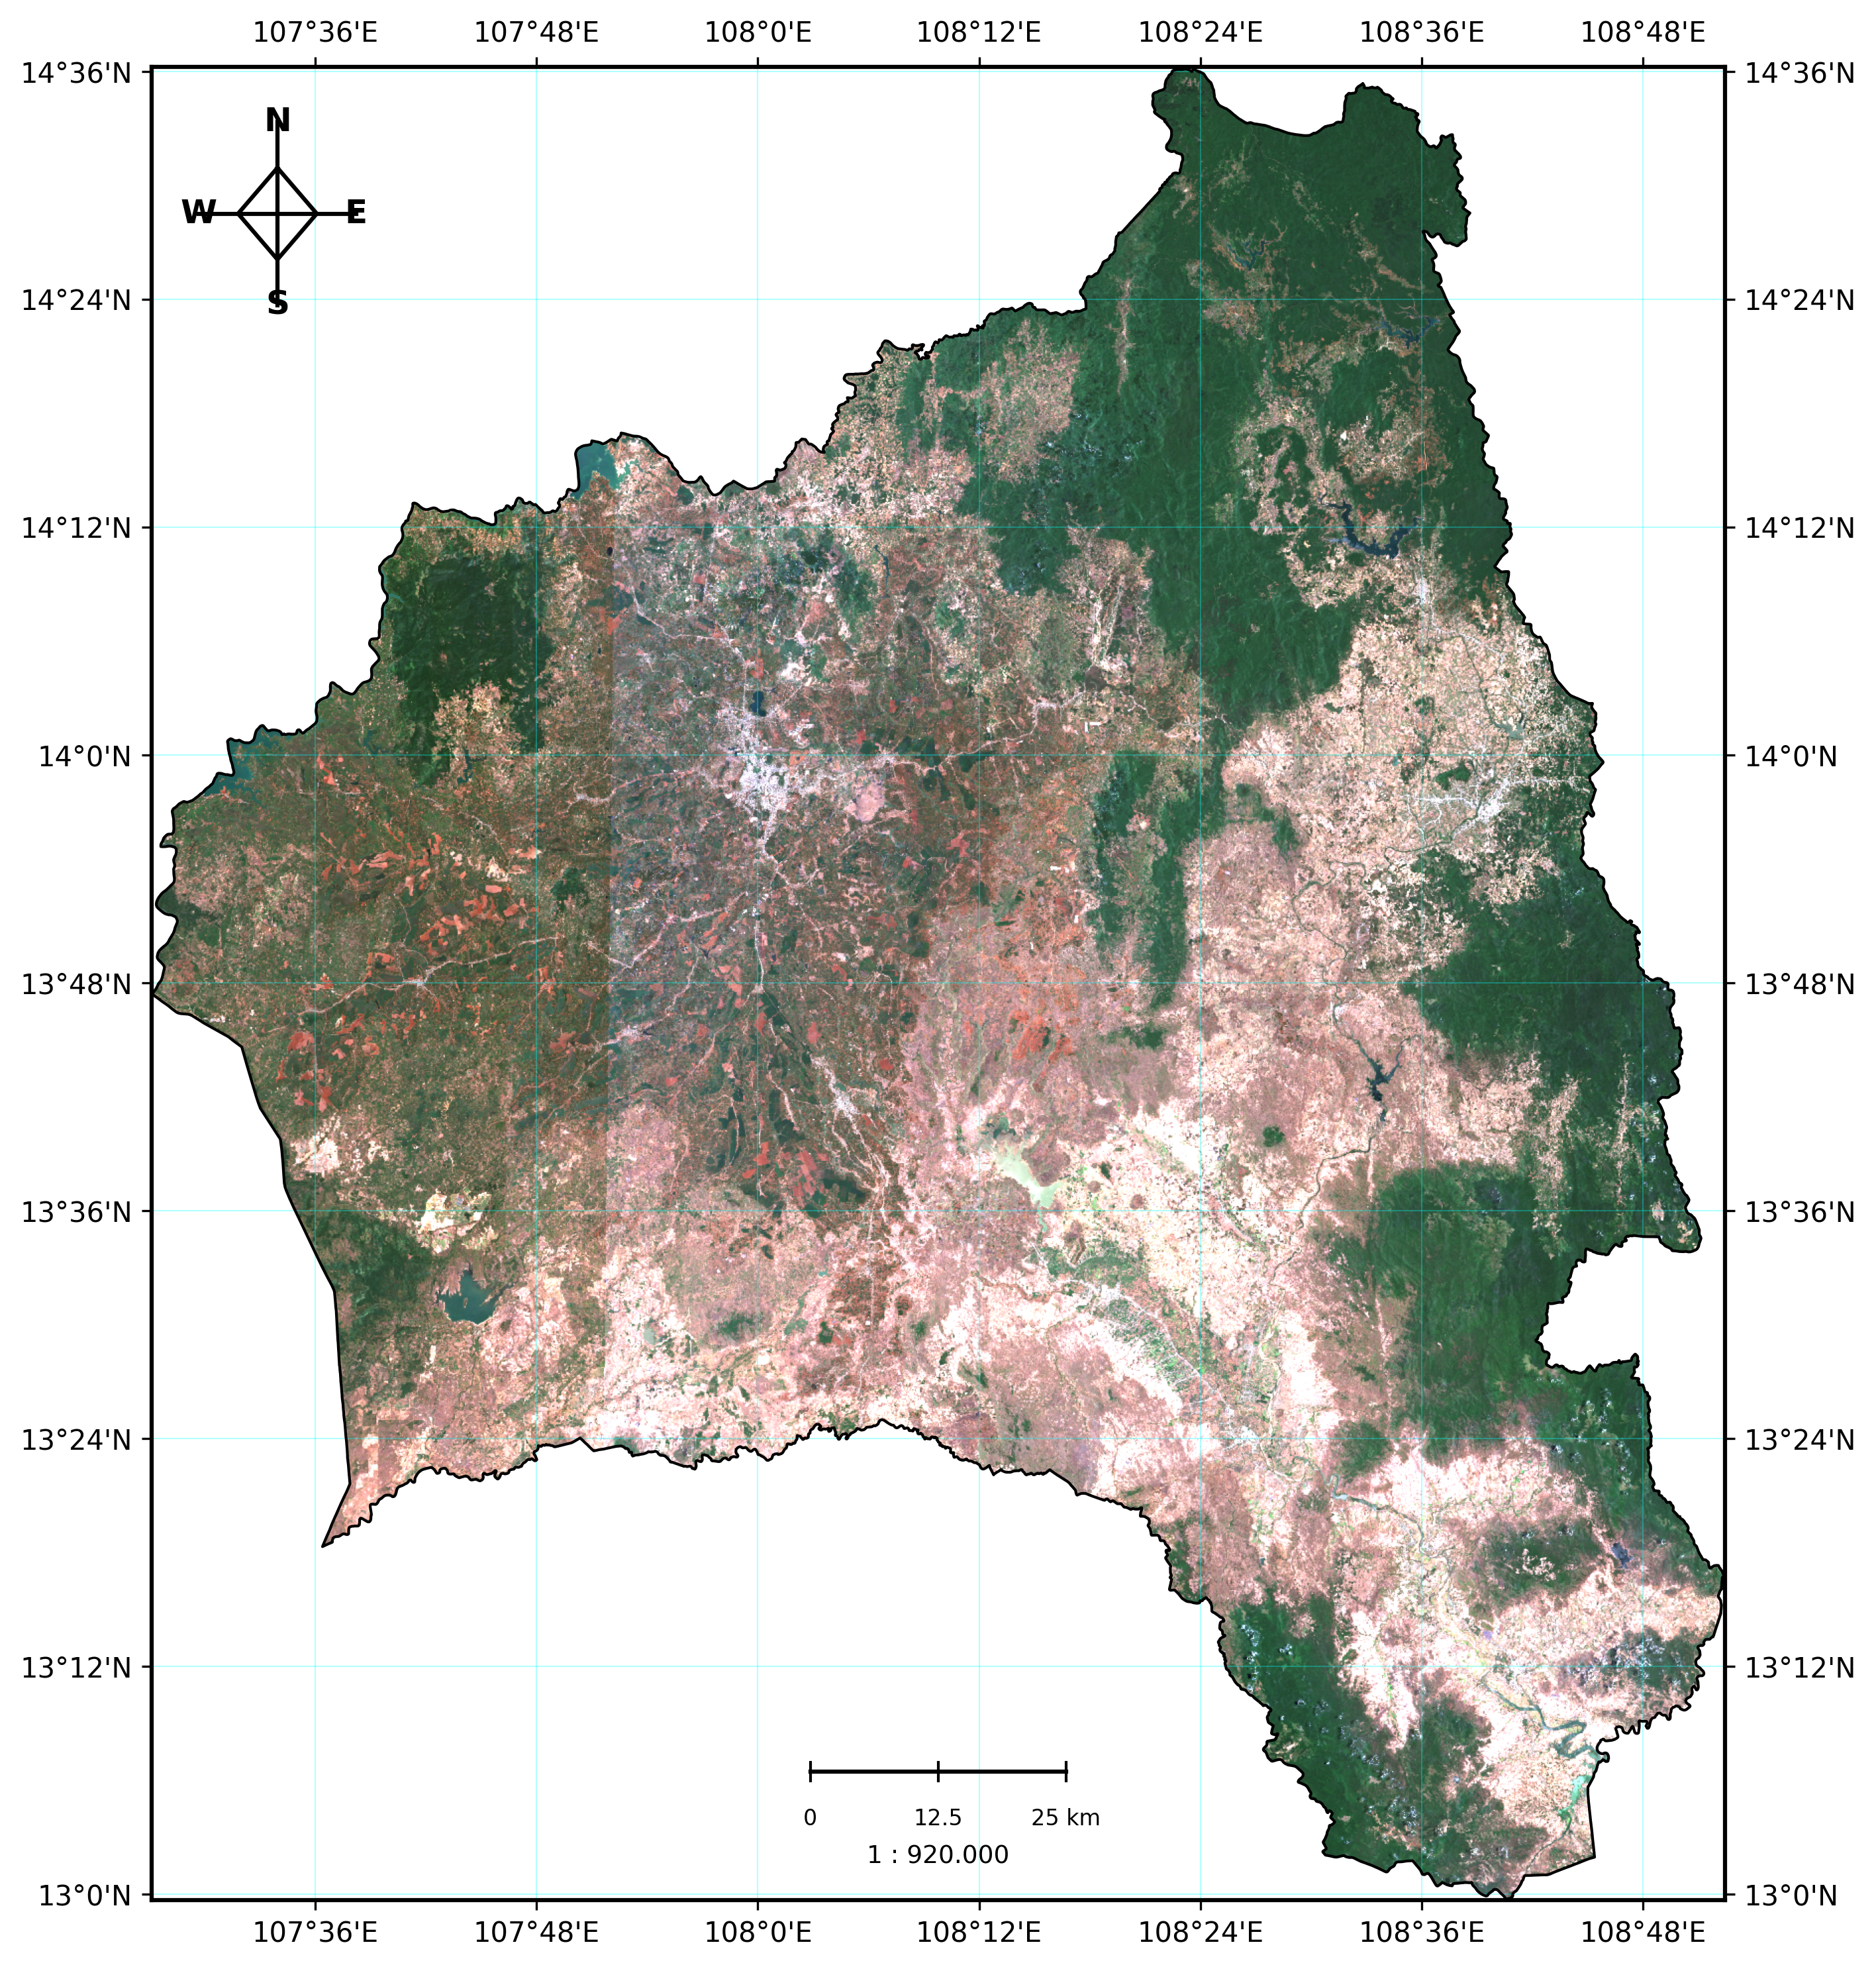
\includegraphics[width=1\textwidth]{TrueColor.png}
\caption{Ảnh màu thực Sentinel-2 tỉnh Gia Lai.}
\label{fig:anh_mau_thuc_sentinel2}
\end{figure}
\FloatBarrier

\subsection{Các Biến Dự báo (Predictor Variables)} % Mục con 3.2: Các Biến Dự báo
Dựa trên các dữ liệu đã thu thập và tổng quan tài liệu, 15 biến dự báo sau đây đã được tính toán và sử dụng để huấn luyện mô hình (tham khảo quy trình trong Hình~\ref{fig:luu_do_quy_trinh}):

\begin{figure}[H]
\centering
\includegraphics[width=1\textwidth]{flowchart.png}
\caption{Lưu đồ quy trình xử lý dữ liệu và xây dựng mô hình dự báo nguy cơ cháy rừng với 15 biến đầu vào, trong đó dữ liệu điểm cháy thực tế được sử dụng để tạo nhãn đánh giá mô hình.}
\label{fig:luu_do_quy_trinh}
\end{figure}
\FloatBarrier

\textbf{Các nhóm chỉ số dự báo được sử dụng trong nghiên cứu:}
\begin{itemize}
    \item \textbf{Chỉ số thực vật (Vegetation Indices):} NDVI (Normalized Difference Vegetation Index), EVI (Enhanced Vegetation Index), SAVI (Soil-Adjusted Vegetation Index), VCI (Vegetation Condition Index), TCI (Temperature Condition Index).
    \item \textbf{Chỉ số nước và ẩm (Water \& Moisture Indices):} NDWI (Normalized Difference Water Index), LSWI (Land Surface Water Index), NDMI (Normalized Difference Moisture Index).
    \item \textbf{Chỉ số cháy/phục hồi (Burn or Recovery Indices):} NBR (Normalized Burn Ratio).
    \item \textbf{Dữ liệu địa hình (Topographic Variables):} DEM (Digital Elevation Model), Slope (Độ dốc), Aspect (Hướng dốc).
    \item \textbf{Dữ liệu khí tượng (Meteorological Variables):} Precipitation (Lượng mưa), Wind speed (Tốc độ gió).
\end{itemize}

\noindent
\begin{minipage}{0.31\textwidth}
    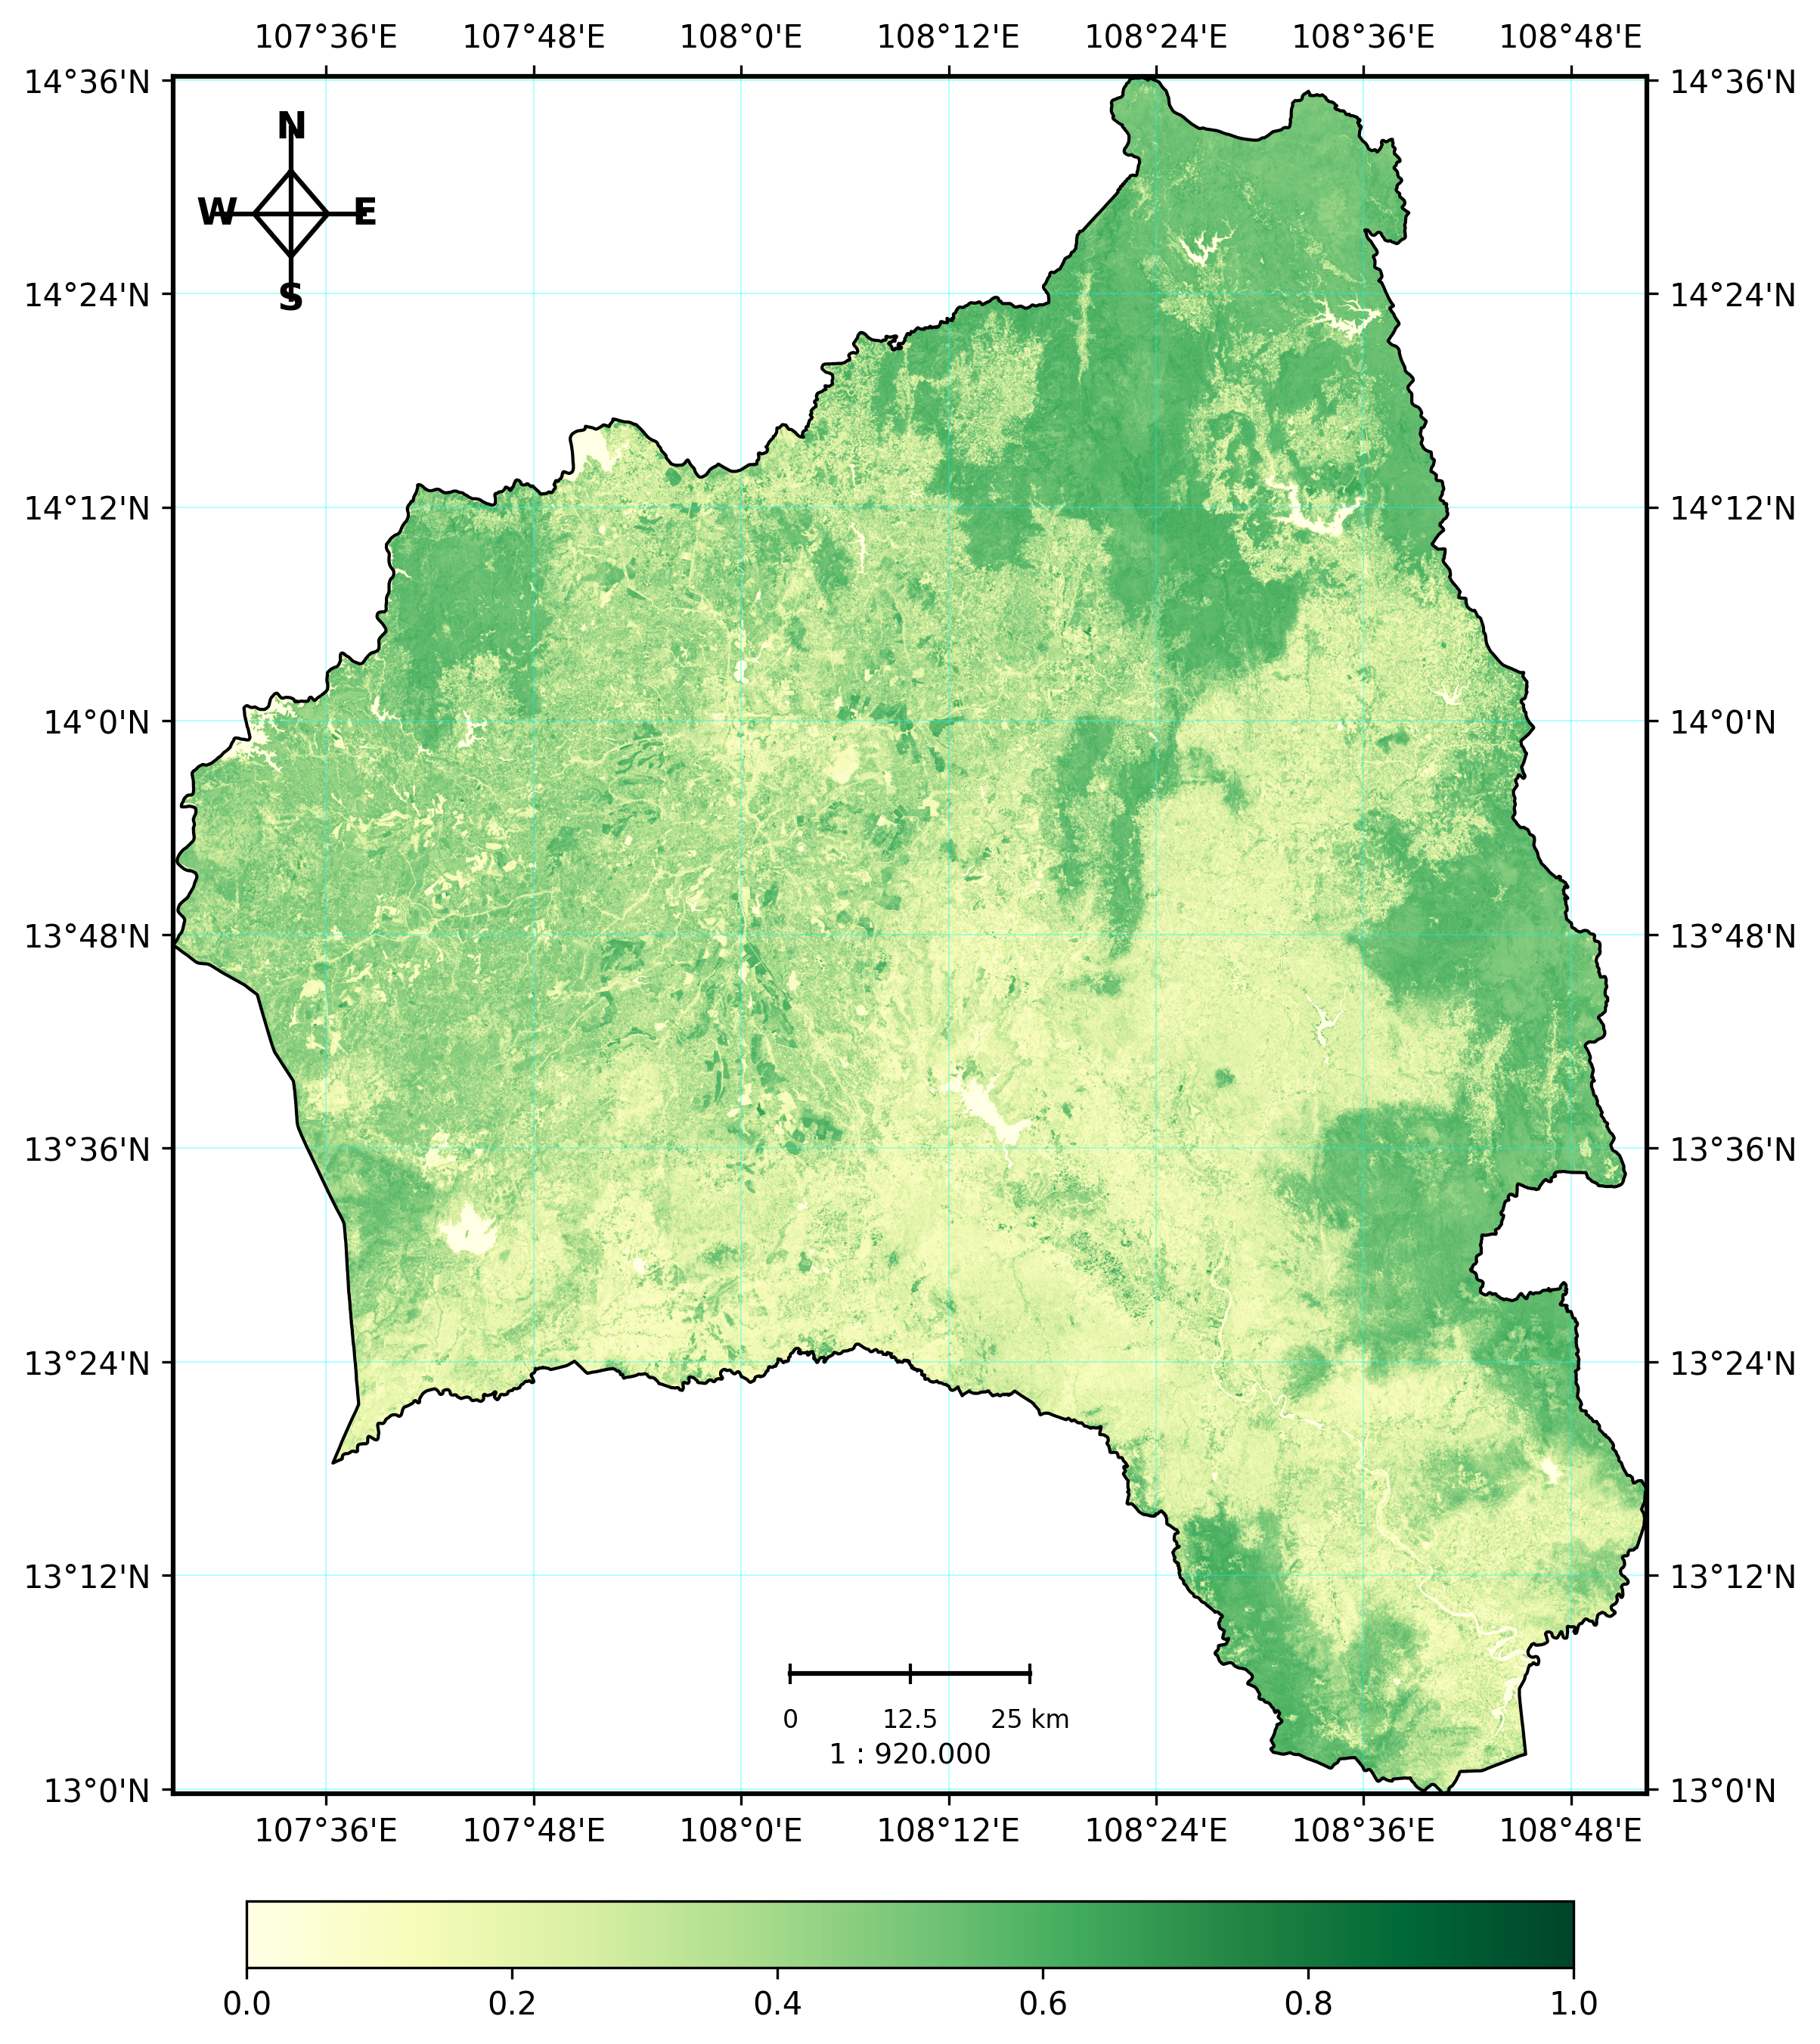
\includegraphics[width=\textwidth]{NDVI.png}
    \centering (a) NDVI
\end{minipage}%
\hfill
\begin{minipage}{0.31\textwidth}
    \includegraphics[width=\textwidth]{EVI.png}
    \centering (b) EVI
\end{minipage}%
\hfill
\begin{minipage}{0.31\textwidth}
    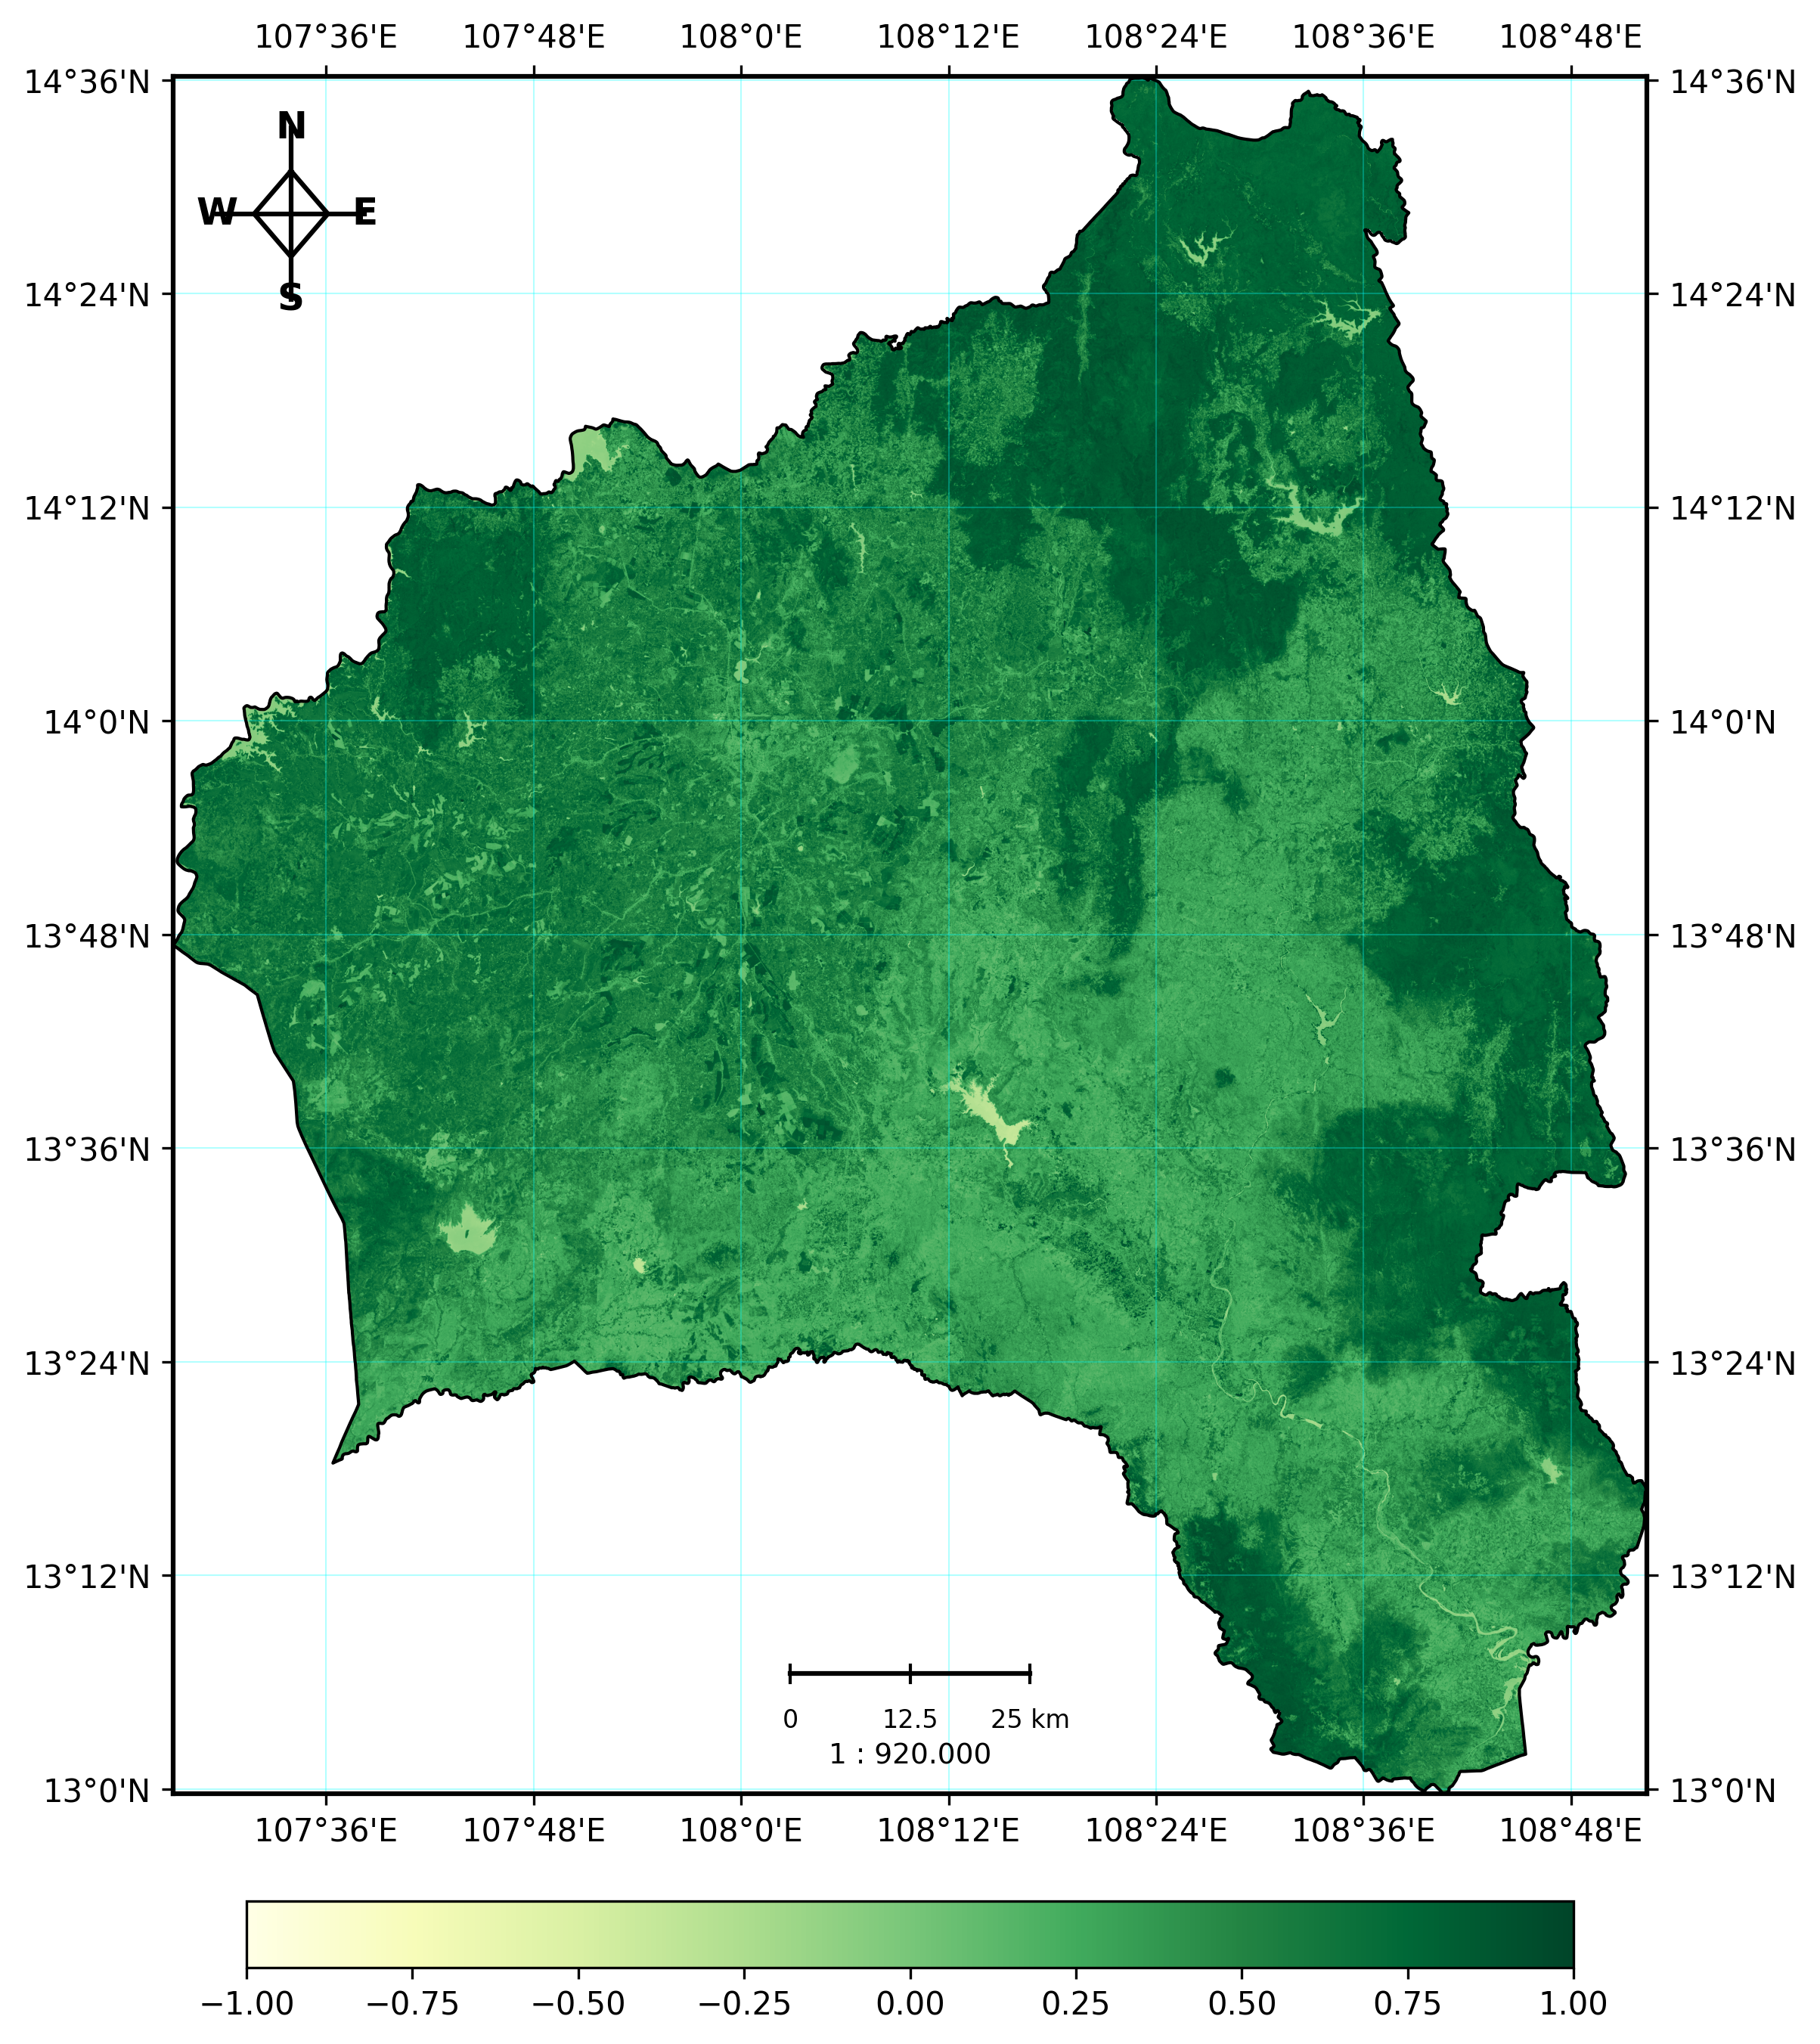
\includegraphics[width=\textwidth]{SAVI.png}
    \centering (c) SAVI
\end{minipage}

\vspace{0.5em}

\noindent
\begin{minipage}{0.31\textwidth}
    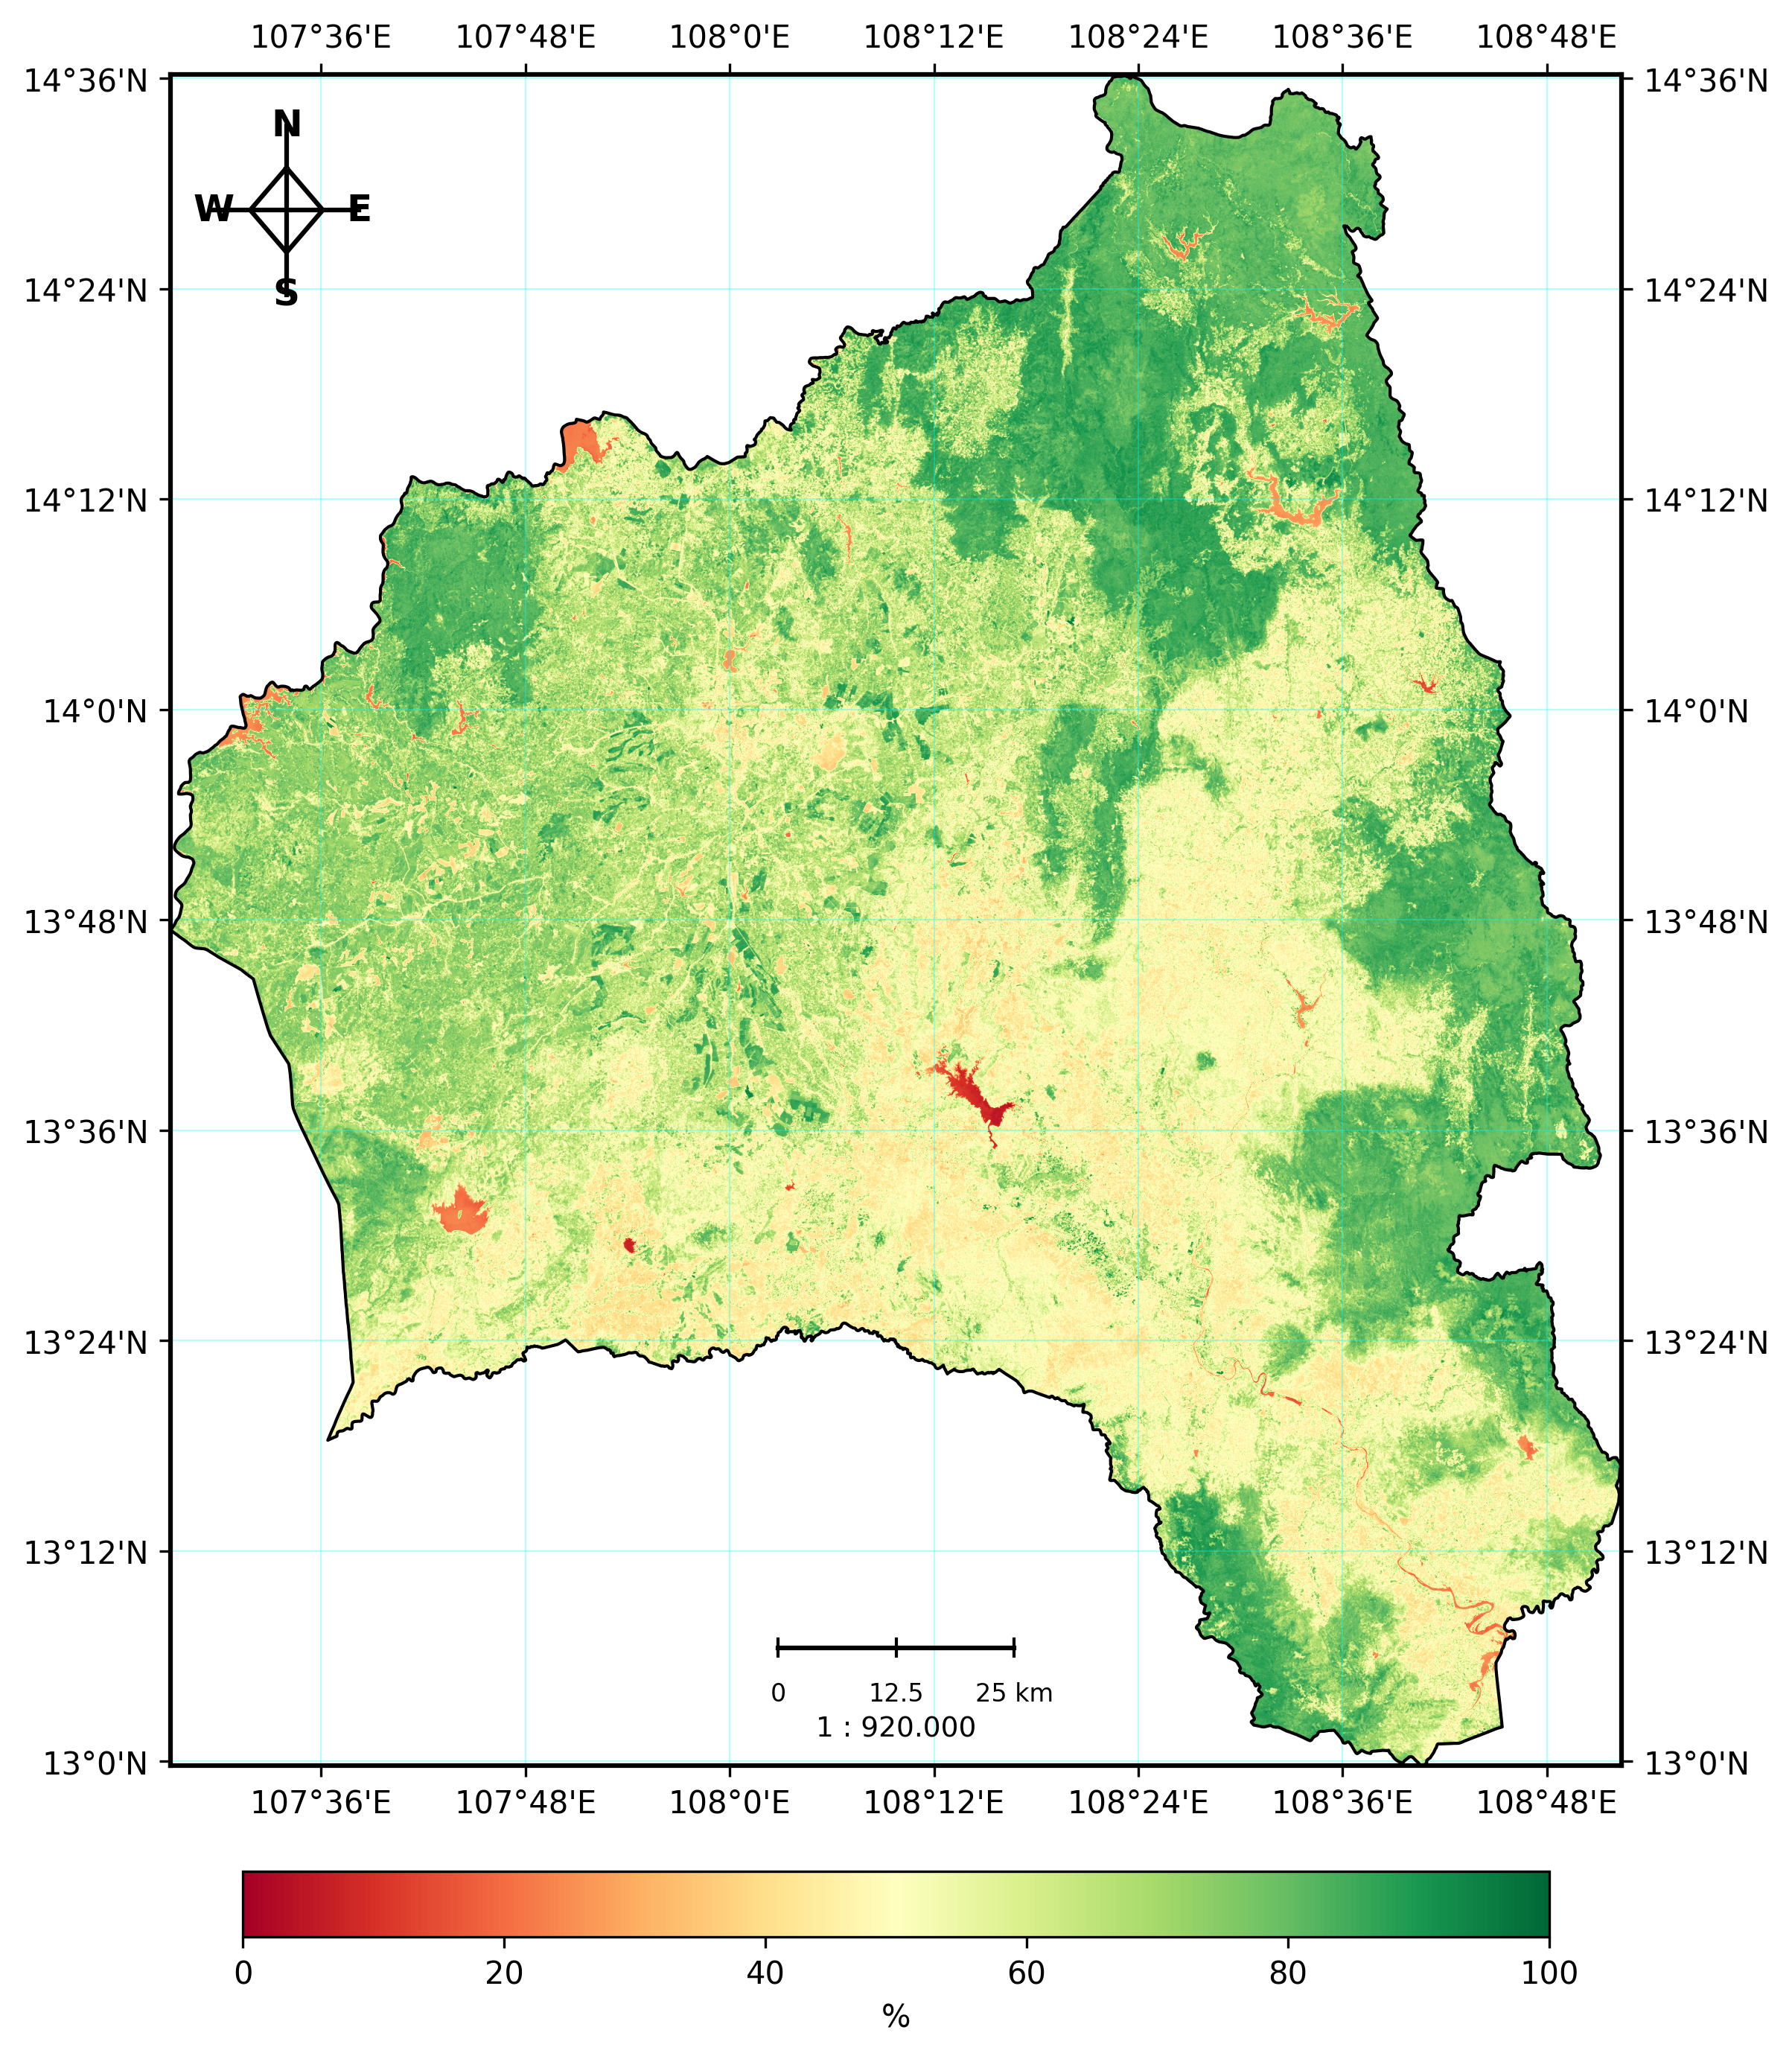
\includegraphics[width=\textwidth]{VCI.png}
    \centering (d) VCI
\end{minipage}%
\hfill
\begin{minipage}{0.31\textwidth}
    \includegraphics[width=\textwidth]{TCI.png}
    \centering (e) TCI
\end{minipage}%
\hfill
\begin{minipage}{0.31\textwidth}
    \includegraphics[width=\textwidth]{NDWI.png}
    \centering (f) NDWI
\end{minipage}

\vspace{0.5em}

\noindent
\begin{minipage}{0.31\textwidth}
    \includegraphics[width=\textwidth]{LSWI.png}
    \centering (g) LSWI
\end{minipage}%
\hfill
\begin{minipage}{0.31\textwidth}
    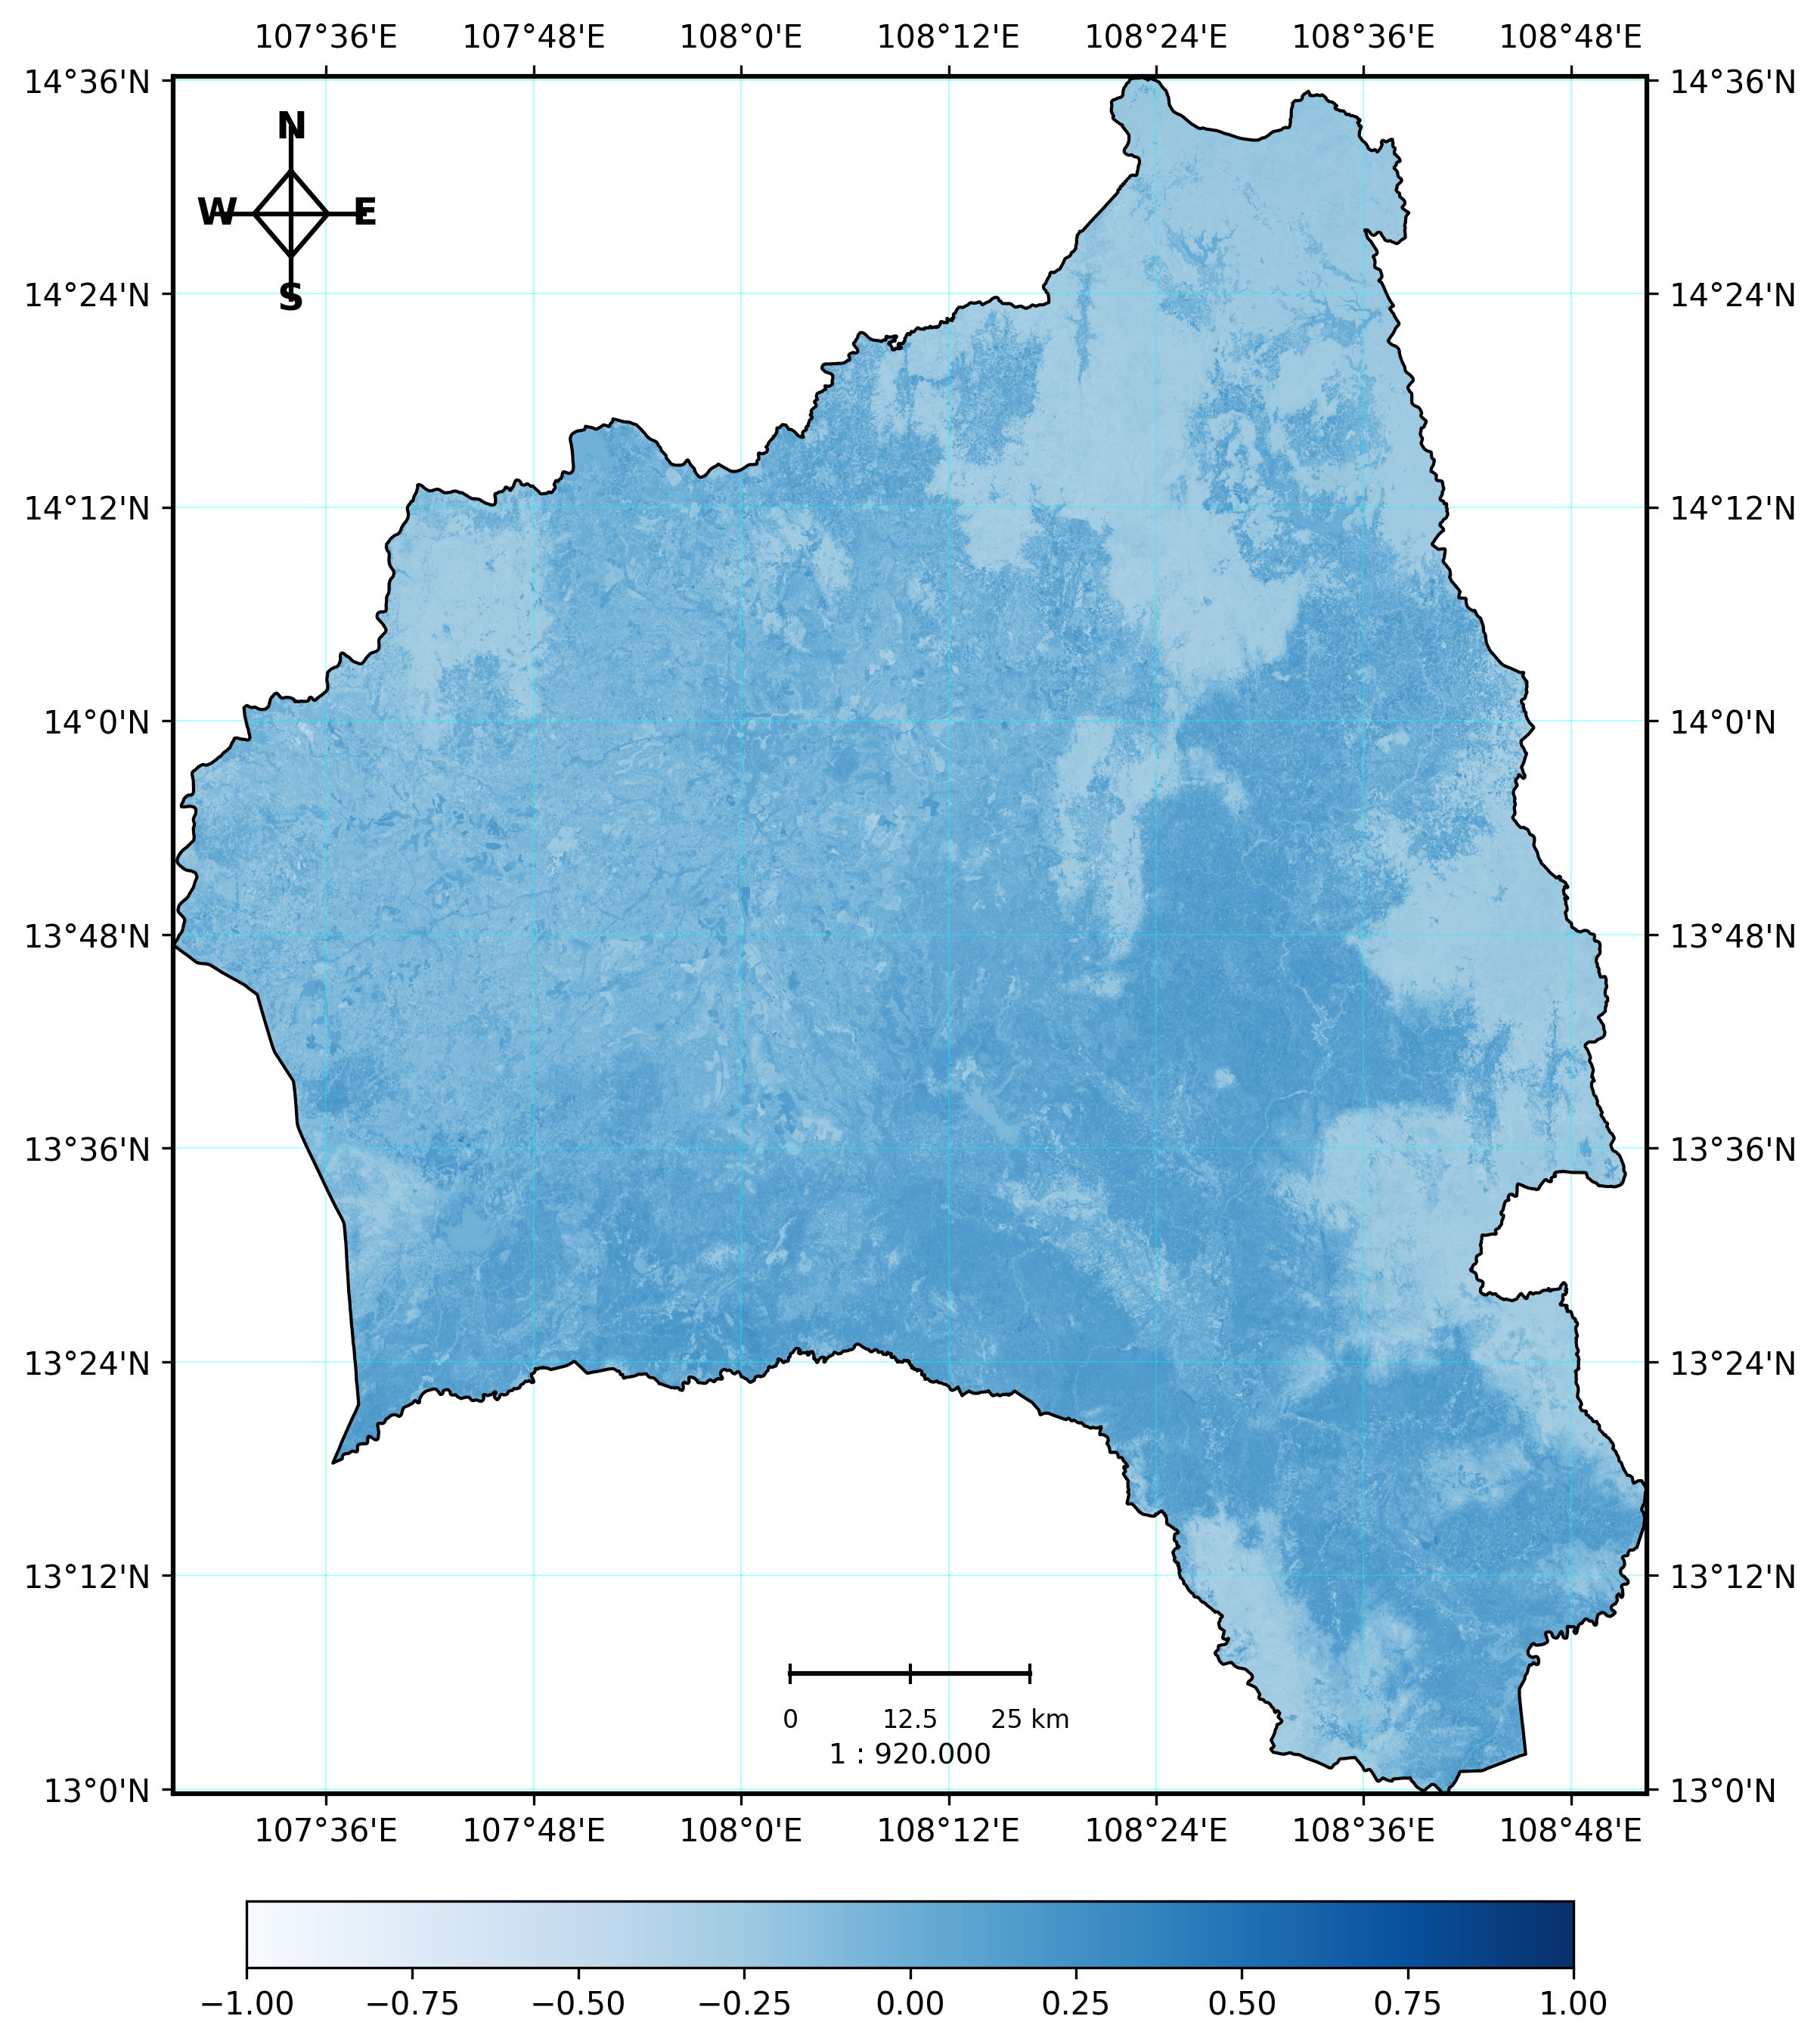
\includegraphics[width=\textwidth]{NDMI.png}
    \centering (h) NDMI
\end{minipage}%
\hfill
\begin{minipage}{0.31\textwidth}
    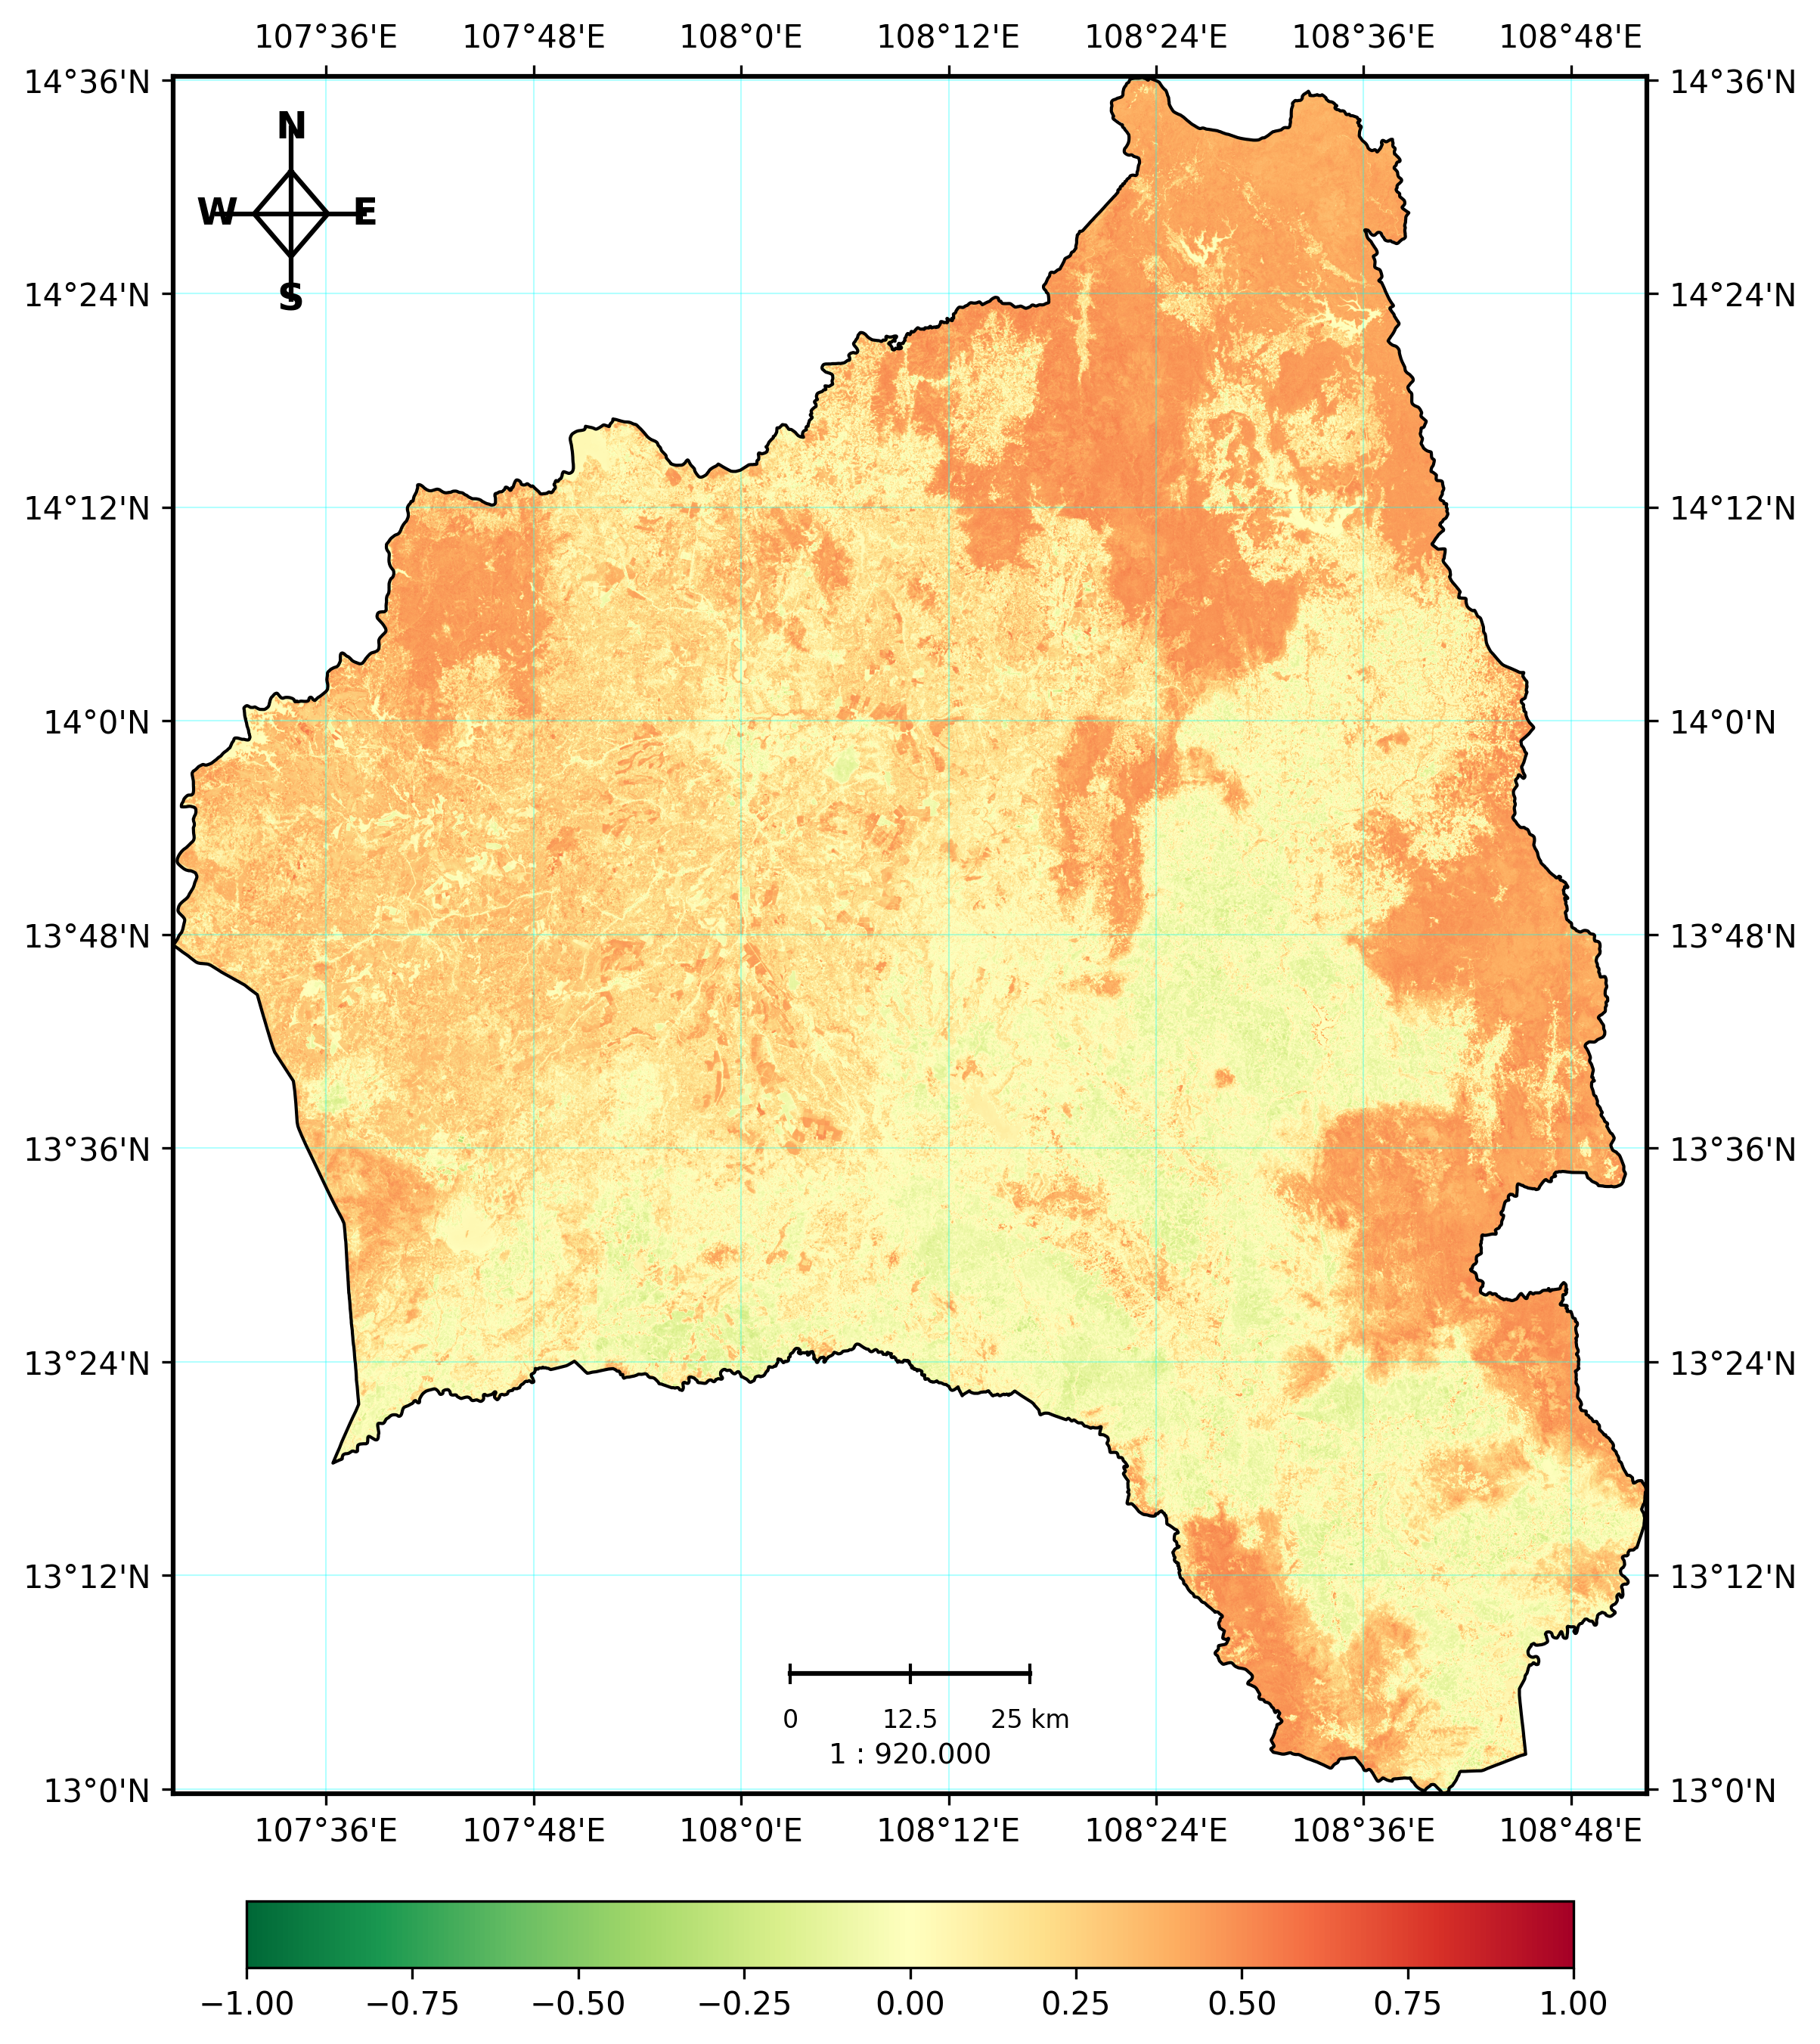
\includegraphics[width=\textwidth]{NBR.png}
    \centering (i) NBR
\end{minipage}

\vspace{0.5em}

\noindent
\begin{minipage}{0.31\textwidth}
    \includegraphics[width=\textwidth]{DEM.png}
    \centering (j) DEM
\end{minipage}%
\hfill
\begin{minipage}{0.31\textwidth}
    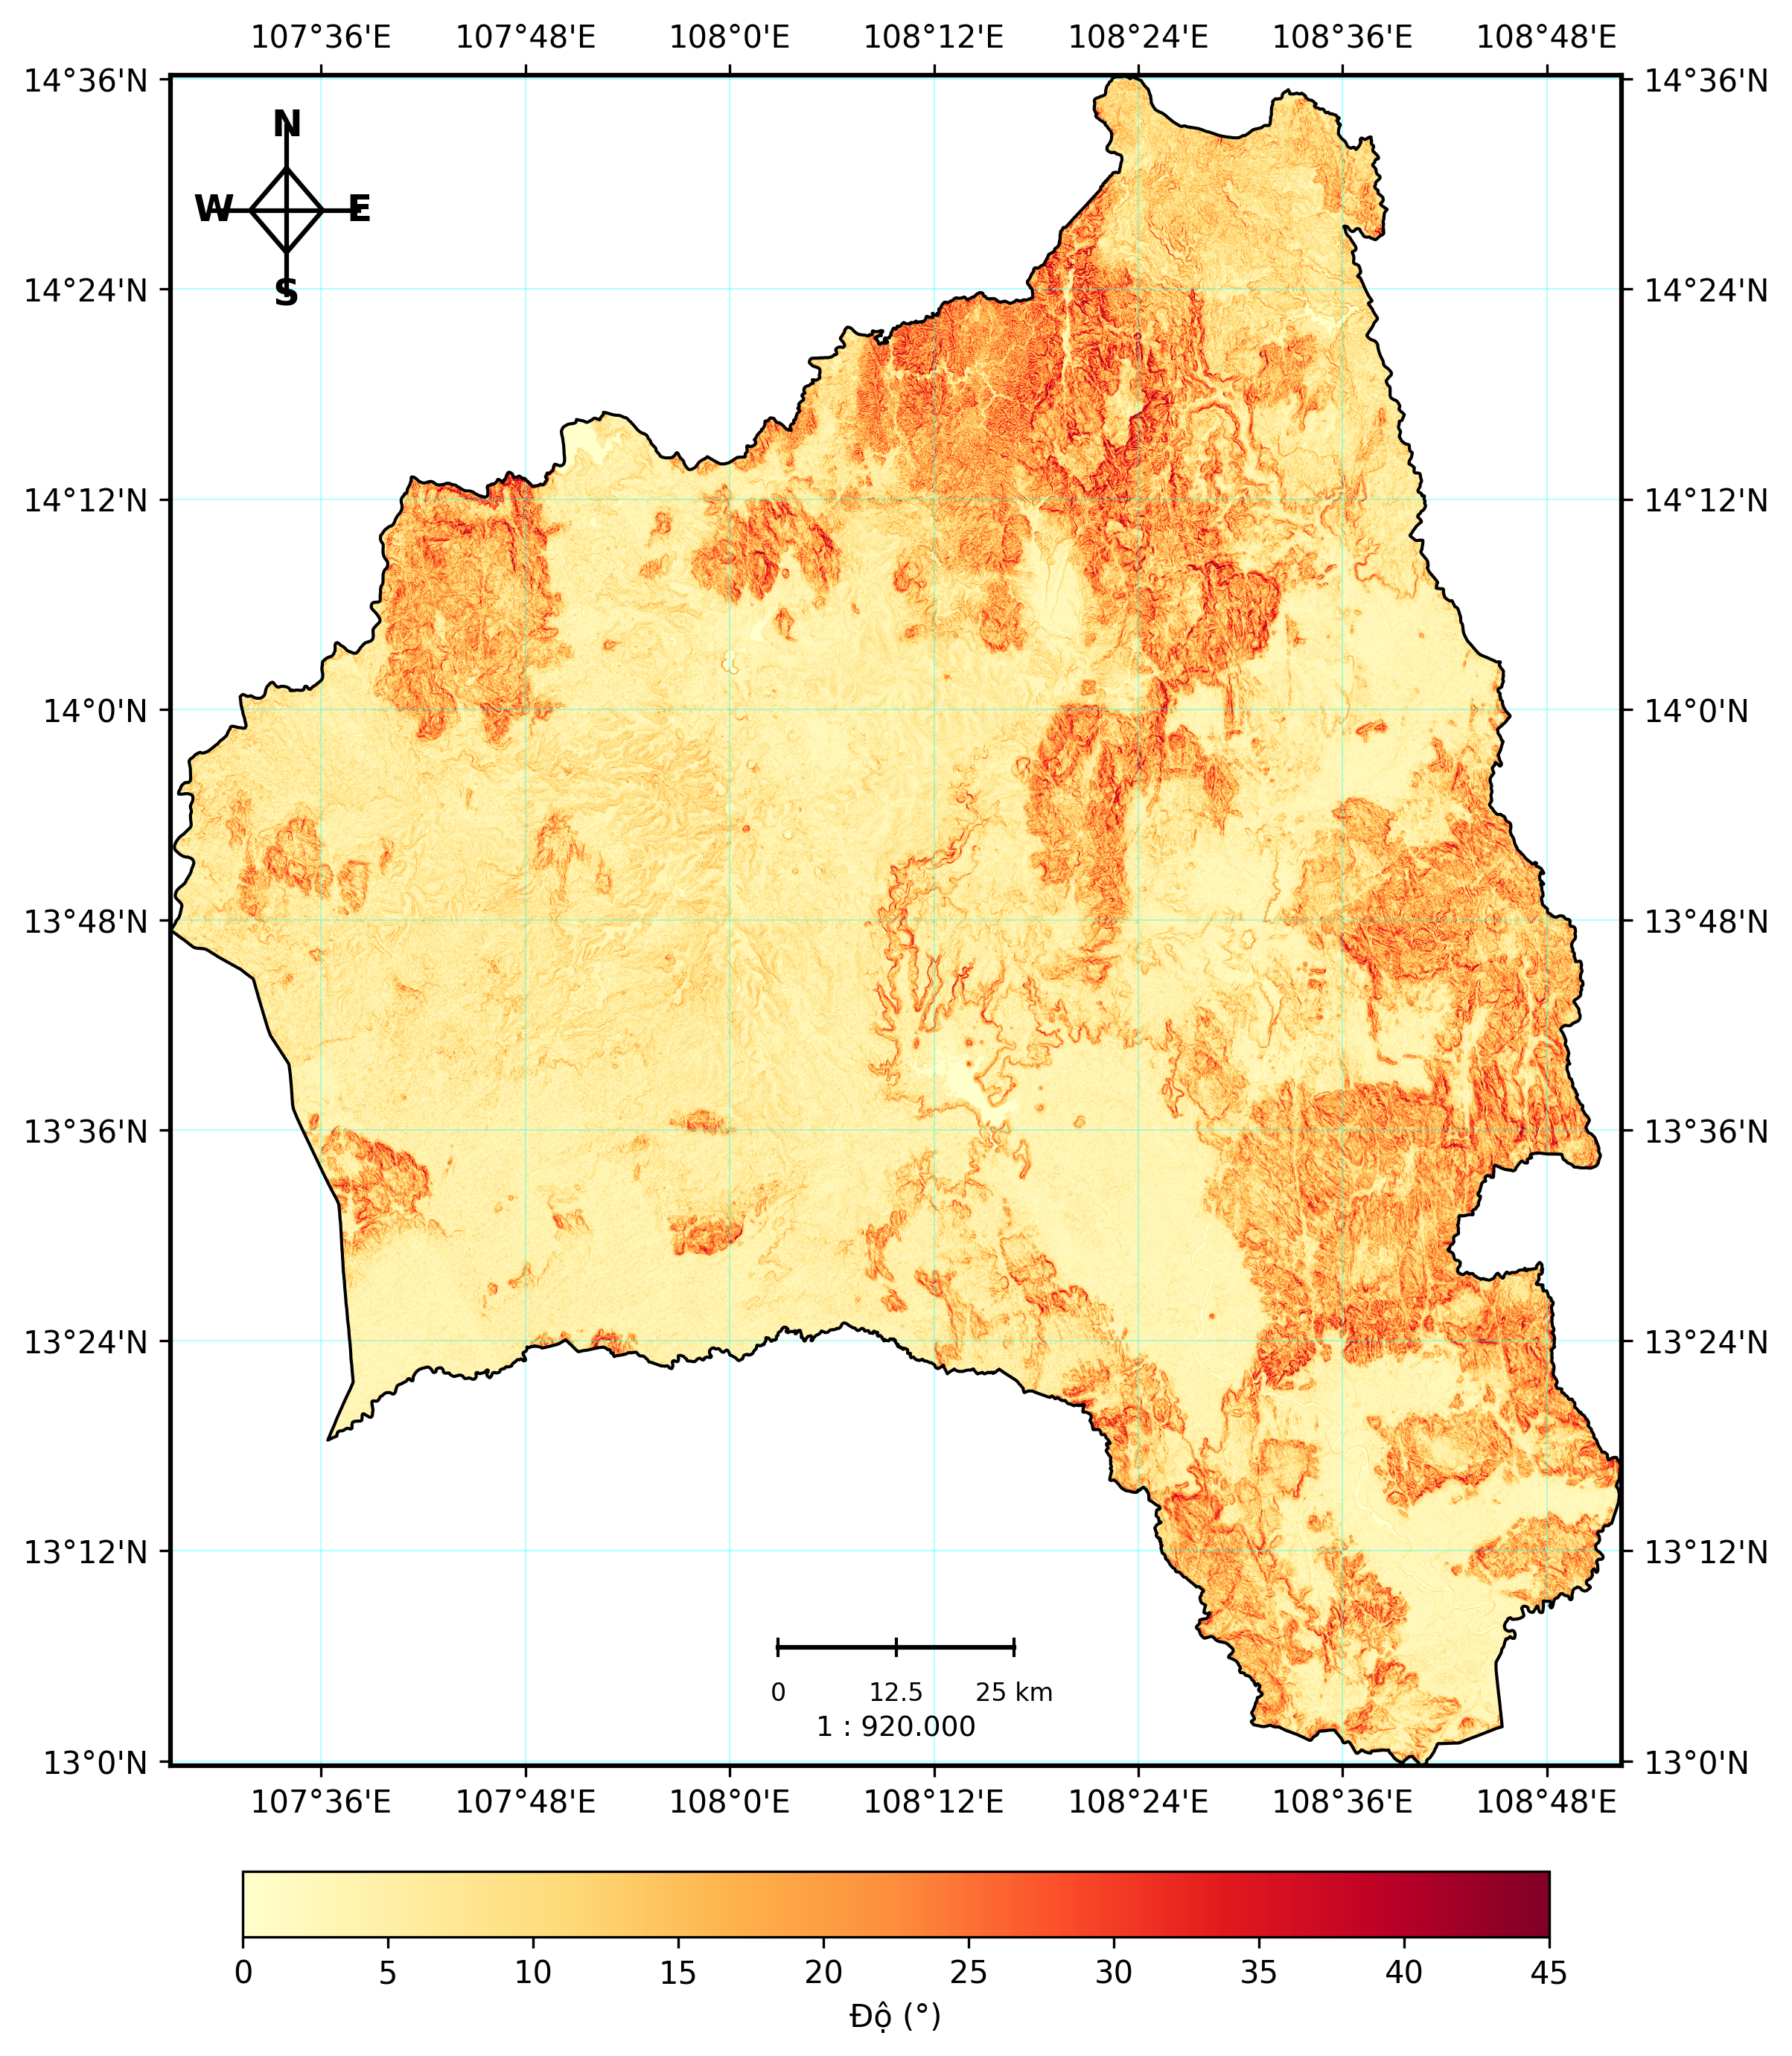
\includegraphics[width=\textwidth]{Slope.png}
    \centering (k) Slope
\end{minipage}%
\hfill
\begin{minipage}{0.31\textwidth}
    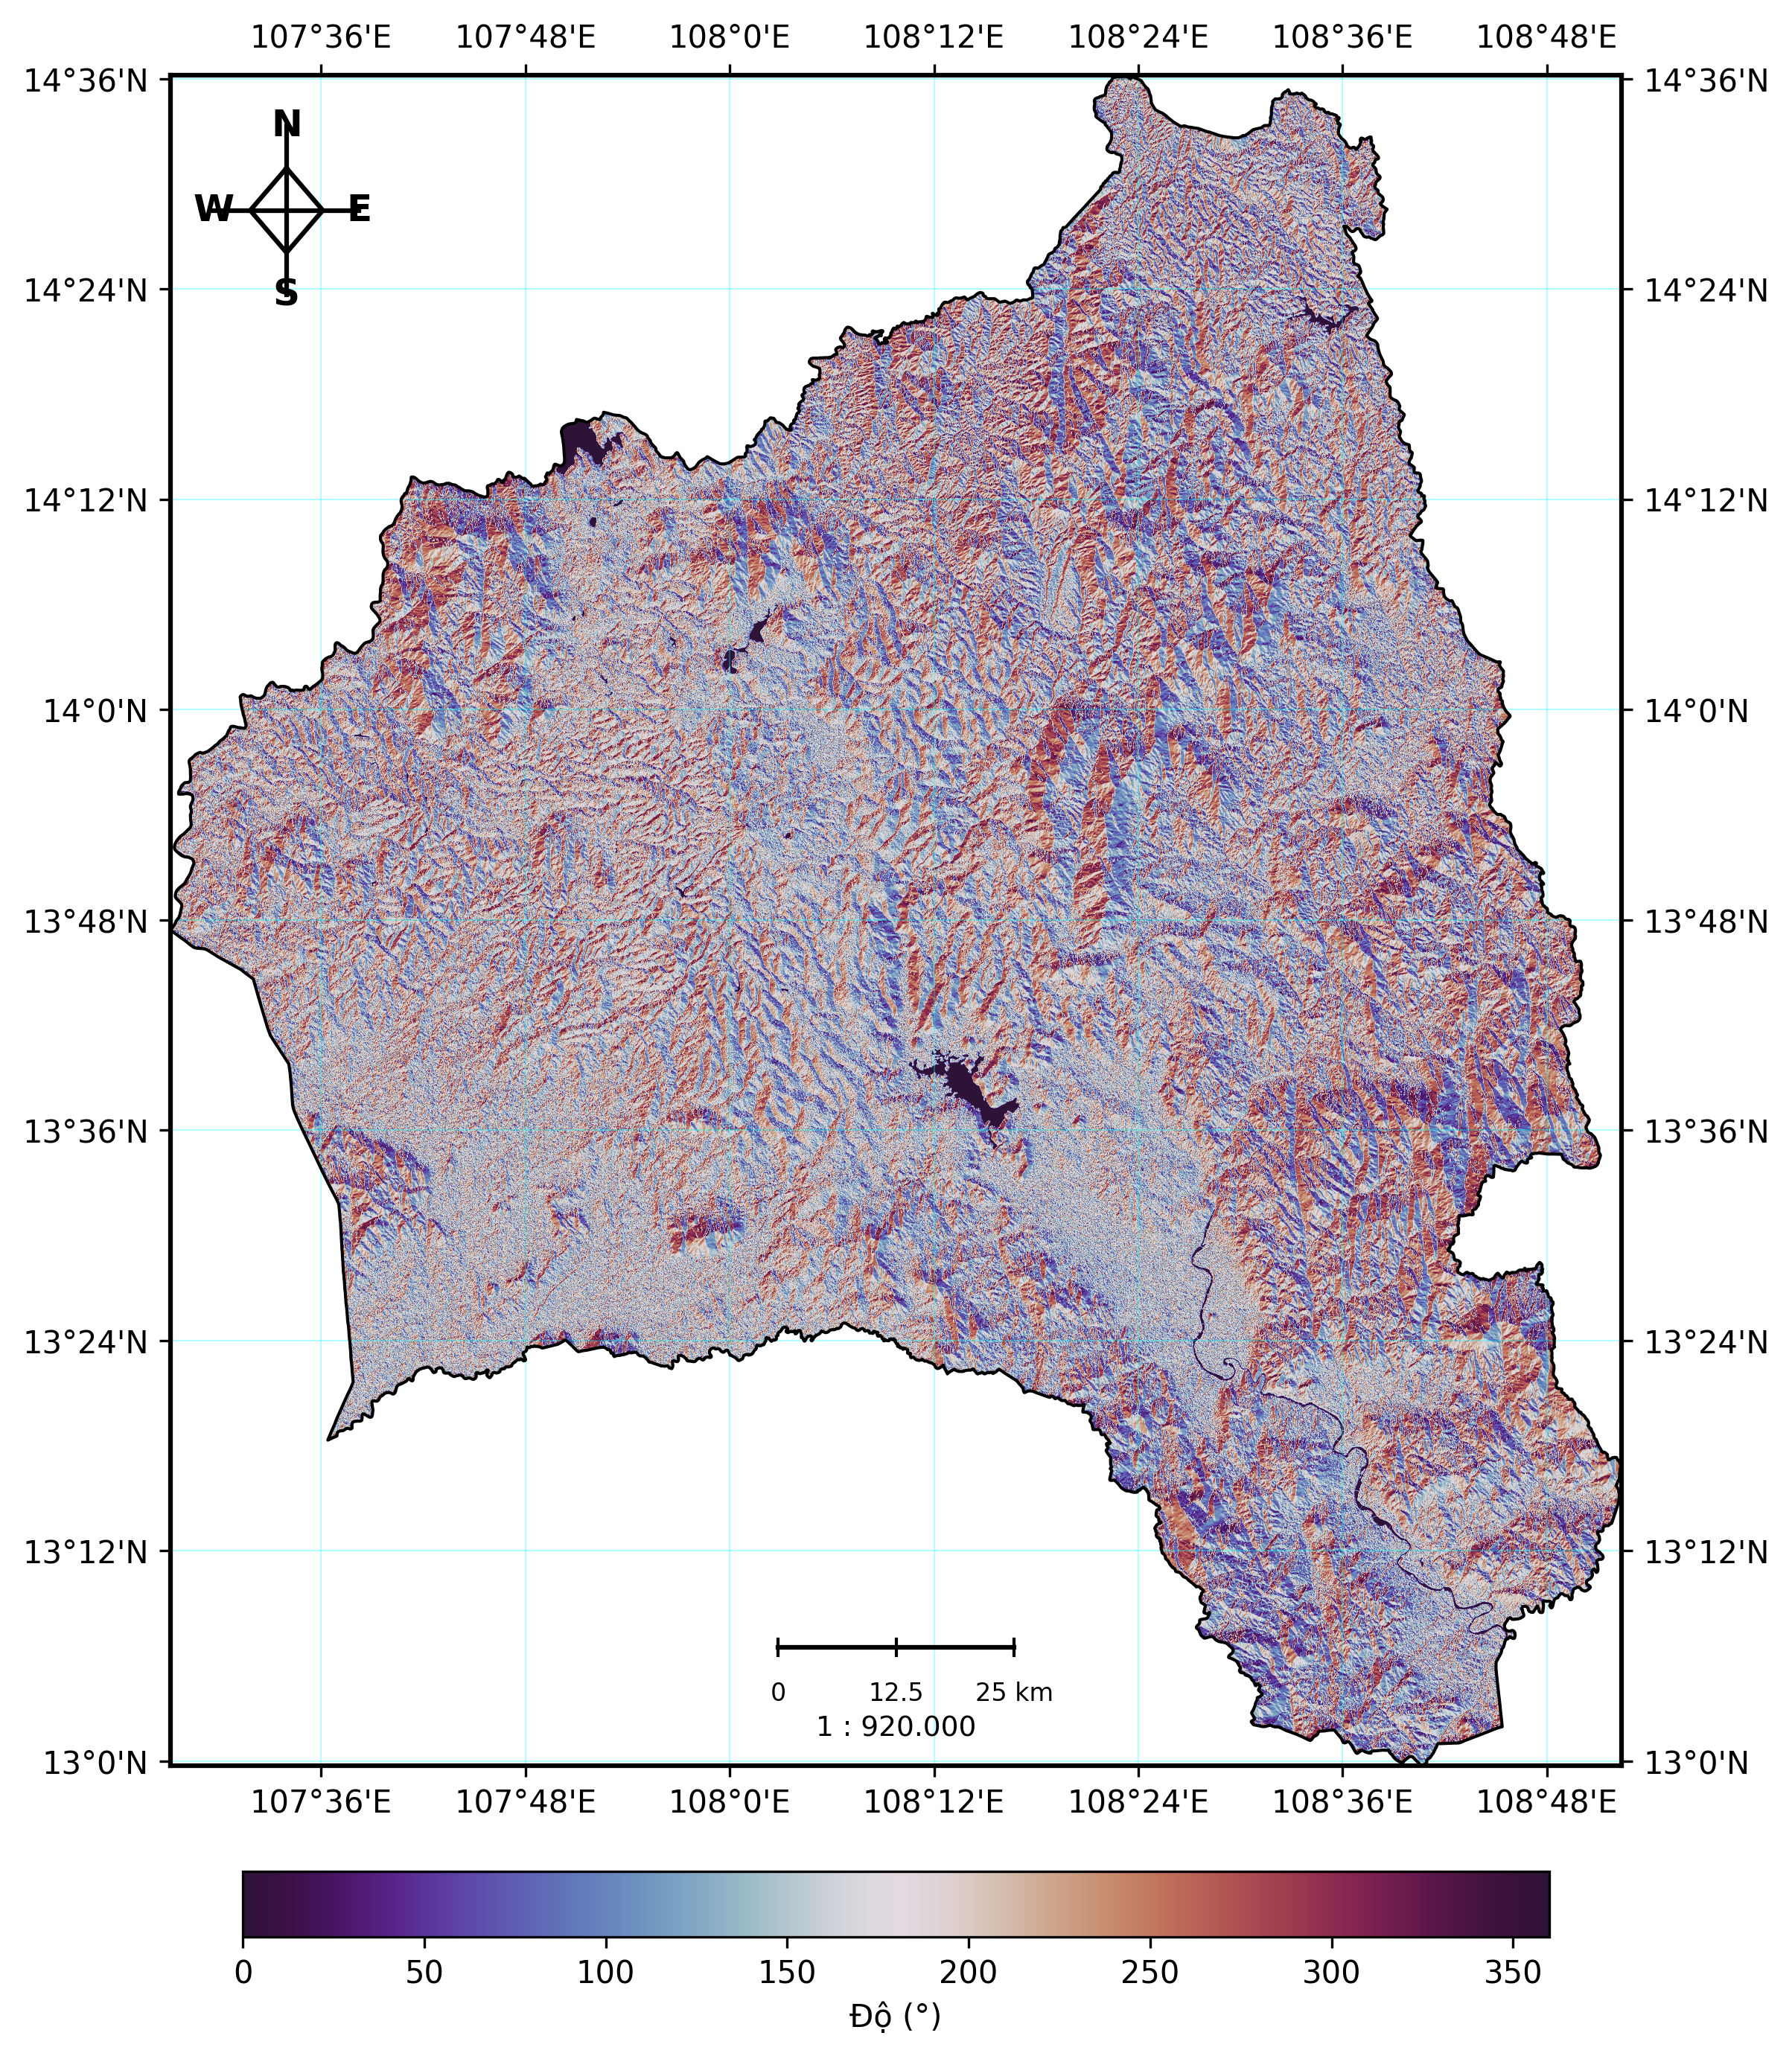
\includegraphics[width=\textwidth]{Aspect.png}
    \centering (l) Aspect
\end{minipage}

\vspace{0.5em}

\noindent
\begin{minipage}{0.31\textwidth}
    \includegraphics[width=\textwidth]{Precipitation.png}
    \centering (m) Precipitation
\end{minipage}%
\hfill
\begin{minipage}{0.31\textwidth}
    \includegraphics[width=\textwidth]{WindSpeed.png}
    \centering (n) Wind speed
\end{minipage}%
\hfill
\begin{minipage}{0.31\textwidth}
    \includegraphics[width=\textwidth]{LST.png}
    \centering (o) LST
\end{minipage}

\vspace{0.5em}

\captionof{figure}{Các bản đồ phân bố không gian của 15 biến đầu vào chính sử dụng trong mô hình dự báo nguy cơ cháy rừng.}
\label{fig:all_predictor_maps}

\noindent
\begin{minipage}{\textwidth}
    \centering
    \includegraphics[width=1\textwidth]{Actual_Fire.png}
    \captionof{figure}{Bản đồ các điểm cháy thực tế từ MODIS được sử dụng làm nhãn để huấn luyện và đánh giá mô hình.}
    \label{fig:diem_chay_thuc_te}
\end{minipage}

\subsection{Xây dựng Mô hình Học máy} % Mục con 3.3: Xây dựng Mô hình Học máy
Quy trình xây dựng mô hình bao gồm các bước sau:
\begin{enumerate}
    \item \textbf{Chuẩn bị dữ liệu:} Tất cả 15 biến đầu vào bao gồm các chỉ số thực vật, độ ẩm, địa hình và khí hậu được chuẩn hóa và kết hợp thành một bộ dữ liệu đa chiều. Dữ liệu điểm cháy từ MODIS \texttt{FireMask} được sử dụng để tạo lớp nhãn cháy (\texttt{Fire\_Label}) cho việc huấn luyện và đánh giá mô hình. Các pixel có giá trị \texttt{FireMask} > 6 được gán nhãn là cháy (1), các pixel khác là không cháy (0).
    \item \textbf{Lấy mẫu dữ liệu:} Để đảm bảo tính nhất quán, tất cả các biến dự báo (sau khi được xử lý ở các độ phân giải gốc hoặc độ phân giải phân tích phù hợp như mô tả ở Mục 3.1, ví dụ: các chỉ số Sentinel ở 10-30m, LST ở 1km, nhãn cháy MODIS ở 500m) và lớp nhãn cháy đã được lấy mẫu thống nhất tại quy mô không gian 500m sử dụng phương pháp \texttt{stratifiedSample} trong Google Earth Engine. Tổng cộng 1000 điểm mẫu đã được thu thập theo cách này, phân tầng theo lớp nhãn cháy (\texttt{Fire\_Label}). Các điểm mẫu này sau đó được chia ngẫu nhiên thành 70\% cho tập huấn luyện (khoảng 700 điểm) và 30\% cho tập kiểm tra (khoảng 300 điểm).
    \item \textbf{Huấn luyện mô hình:} Hai thuật toán học máy là Random Forest (RF) và Gradient Tree Boosting (GTB) được huấn luyện. 
        Đối với Random Forest (RF), các tham số chính được sử dụng trong Google Earth Engine bao gồm: \texttt{numberOfTrees} = 100 (Số lượng cây trong rừng), \texttt{minLeafPopulation} = 5 (Số lượng mẫu tối thiểu tại một nút lá), \texttt{bagFraction} = 0.7 (Tỷ lệ mẫu con cho mỗi cây), và \texttt{seed} = 42 (Giá trị khởi tạo cho bộ sinh số ngẫu nhiên).
        Đối với Gradient Tree Boosting (GTB), các tham số chính được sử dụng bao gồm: \texttt{numberOfTrees} = 100 (Số lượng cây), \texttt{shrinkage} = 0.05 (Tốc độ học), \texttt{samplingRate} = 0.7 (Tỷ lệ mẫu con của dữ liệu đầu vào), \texttt{maxNodes} = 10 (Số lượng nút tối đa cho mỗi cây), và \texttt{seed} = 42.
        Mô hình được huấn luyện ở chế độ \texttt{PROBABILITY} để tạo bản đồ xác suất và \texttt{CLASSIFICATION} để đánh giá độ chính xác trên tập kiểm tra.
    \item \textbf{Tạo bản đồ dự đoán:} Các mô hình đã huấn luyện sau đó được áp dụng lên một chồng dữ liệu các biến dự báo đầu vào. Chồng dữ liệu này đã được đồng nhất về độ phân giải không gian 30m (sử dụng phương pháp nội suy song tuyến tính - bilinear interpolation) để tạo ra các bản đồ nguy cơ cháy rừng cuối cùng với độ phân giải 30m.
\end{enumerate}

\subsection{Đánh giá Mô hình} % Mục con 3.4: Đánh giá Mô hình
Hiệu suất của các mô hình được đánh giá trên tập dữ liệu kiểm tra (30\% dữ liệu mẫu) bằng cách sử dụng ma trận nhầm lẫn (Confusion Matrix) và các chỉ số thống kê bao gồm: Độ chính xác tổng thể (Overall Accuracy), Độ chính xác cho lớp cháy (Precision), Độ nhạy cho lớp cháy (Recall), và F1-Score cho lớp cháy.
Ngoài ra, để đánh giá thêm khả năng tổng quát hóa của mô hình, kiểm định chéo 5-fold (5-fold cross-validation) cũng đã được thực hiện trên tập dữ liệu huấn luyện (70\% dữ liệu mẫu, có khả năng sử dụng dữ liệu đã được xuất ra và xử lý bằng một quy trình bên ngoài Google Earth Engine). Kết quả của kiểm định chéo này cũng được sử dụng để so sánh hiệu suất giữa hai mô hình.

\section{Kết quả} % Bắt đầu Mục 4: Kết quả

\subsection{Hiệu suất Mô hình} % Mục con 4.1: Hiệu suất Mô hình
Kết quả đánh giá hiệu suất của hai mô hình được trình bày trong Bảng~\ref{tab:ma_tran_nham_lan_rf}, Bảng~\ref{tab:ma_tran_nham_lan_gtb} và Bảng~\ref{tab:so_sanh_hieu_suat_rf_gtb}.

\begin{table}[H]
\centering
\caption{Ma trận nhầm lẫn (Confusion Matrix) cho mô hình Random Forest (RF) trên tập kiểm tra.}
\label{tab:ma_tran_nham_lan_rf}
\begin{tabular}{>{\bfseries}lcc}
\toprule
& \textbf{Dự đoán Không cháy} & \textbf{Dự đoán Cháy} \\
\midrule
Thực tế Không cháy & 254 (TN) & 79 (FP) \\
Thực tế Cháy       & 64 (FN)  & 250 (TP) \\
\bottomrule
\end{tabular}
\end{table}

\begin{table}[H]
\centering
\caption{Ma trận nhầm lẫn (Confusion Matrix) cho mô hình Gradient Tree Boosting (GTB) trên tập kiểm tra.}
\label{tab:ma_tran_nham_lan_gtb}
\begin{tabular}{>{\bfseries}lcc}
\toprule
& \textbf{Dự đoán Không cháy} & \textbf{Dự đoán Cháy} \\
\midrule
Thực tế Không cháy & 258 (TN) & 75 (FP) \\
Thực tế Cháy       & 72 (FN)  & 242 (TP) \\
\bottomrule
\end{tabular}
\end{table}

\begin{table}[H]
\centering
\caption{So sánh các chỉ số đánh giá hiệu suất của mô hình RF và GTB.}
\label{tab:so_sanh_hieu_suat_rf_gtb}
\begin{tabular}{>{\bfseries}lcc}
\toprule
\textbf{Chỉ số đánh giá} & \textbf{Random Forest} & \textbf{Gradient Tree Boosting} \\
\midrule
Overall Accuracy        & 93.05\%       & 83.81\%                \\
Recall (Lớp Cháy)       & 0.9344        & 0.8455                 \\
Precision (Lớp Cháy)    & 0.9290        & 0.8369                 \\
F1-Score (Lớp Cháy)     & 0.9317        & 0.8412                 \\
Cross-validation (5-fold) & 77.90\% & 77.28\%       \\
\bottomrule
\end{tabular}
\end{table}

\begin{figure}[H]
\centering
\includegraphics[width=0.9\textwidth]{Model_Metrics.png}
\caption{So sánh các chỉ số đánh giá hiệu suất giữa mô hình Random Forest và Gradient Tree Boosting.}
\label{fig:so_sanh_hieu_suat_rf_gtb_bieu_do}
\end{figure}
\FloatBarrier

\subsection{Bản đồ Nguy cơ Cháy rừng} % Mục con 4.2: Bản đồ Nguy cơ Cháy rừng
Bản đồ dự đoán nguy cơ cháy rừng cho tỉnh Gia Lai, được tạo ra từ mô hình RF và GTB, được trình bày trong Hình~\ref{fig:ban_do_nguy_co_rf} và Hình~\ref{fig:ban_do_nguy_co_gtb}.

\begin{figure}[H]
\centering
\includegraphics[width=1\textwidth]{RF_Risk.png}
\caption{Bản đồ dự đoán nguy cơ cháy rừng tỉnh Gia Lai sử dụng mô hình Random Forest.}
\label{fig:ban_do_nguy_co_rf}
\end{figure}

\begin{figure}[H]
\centering
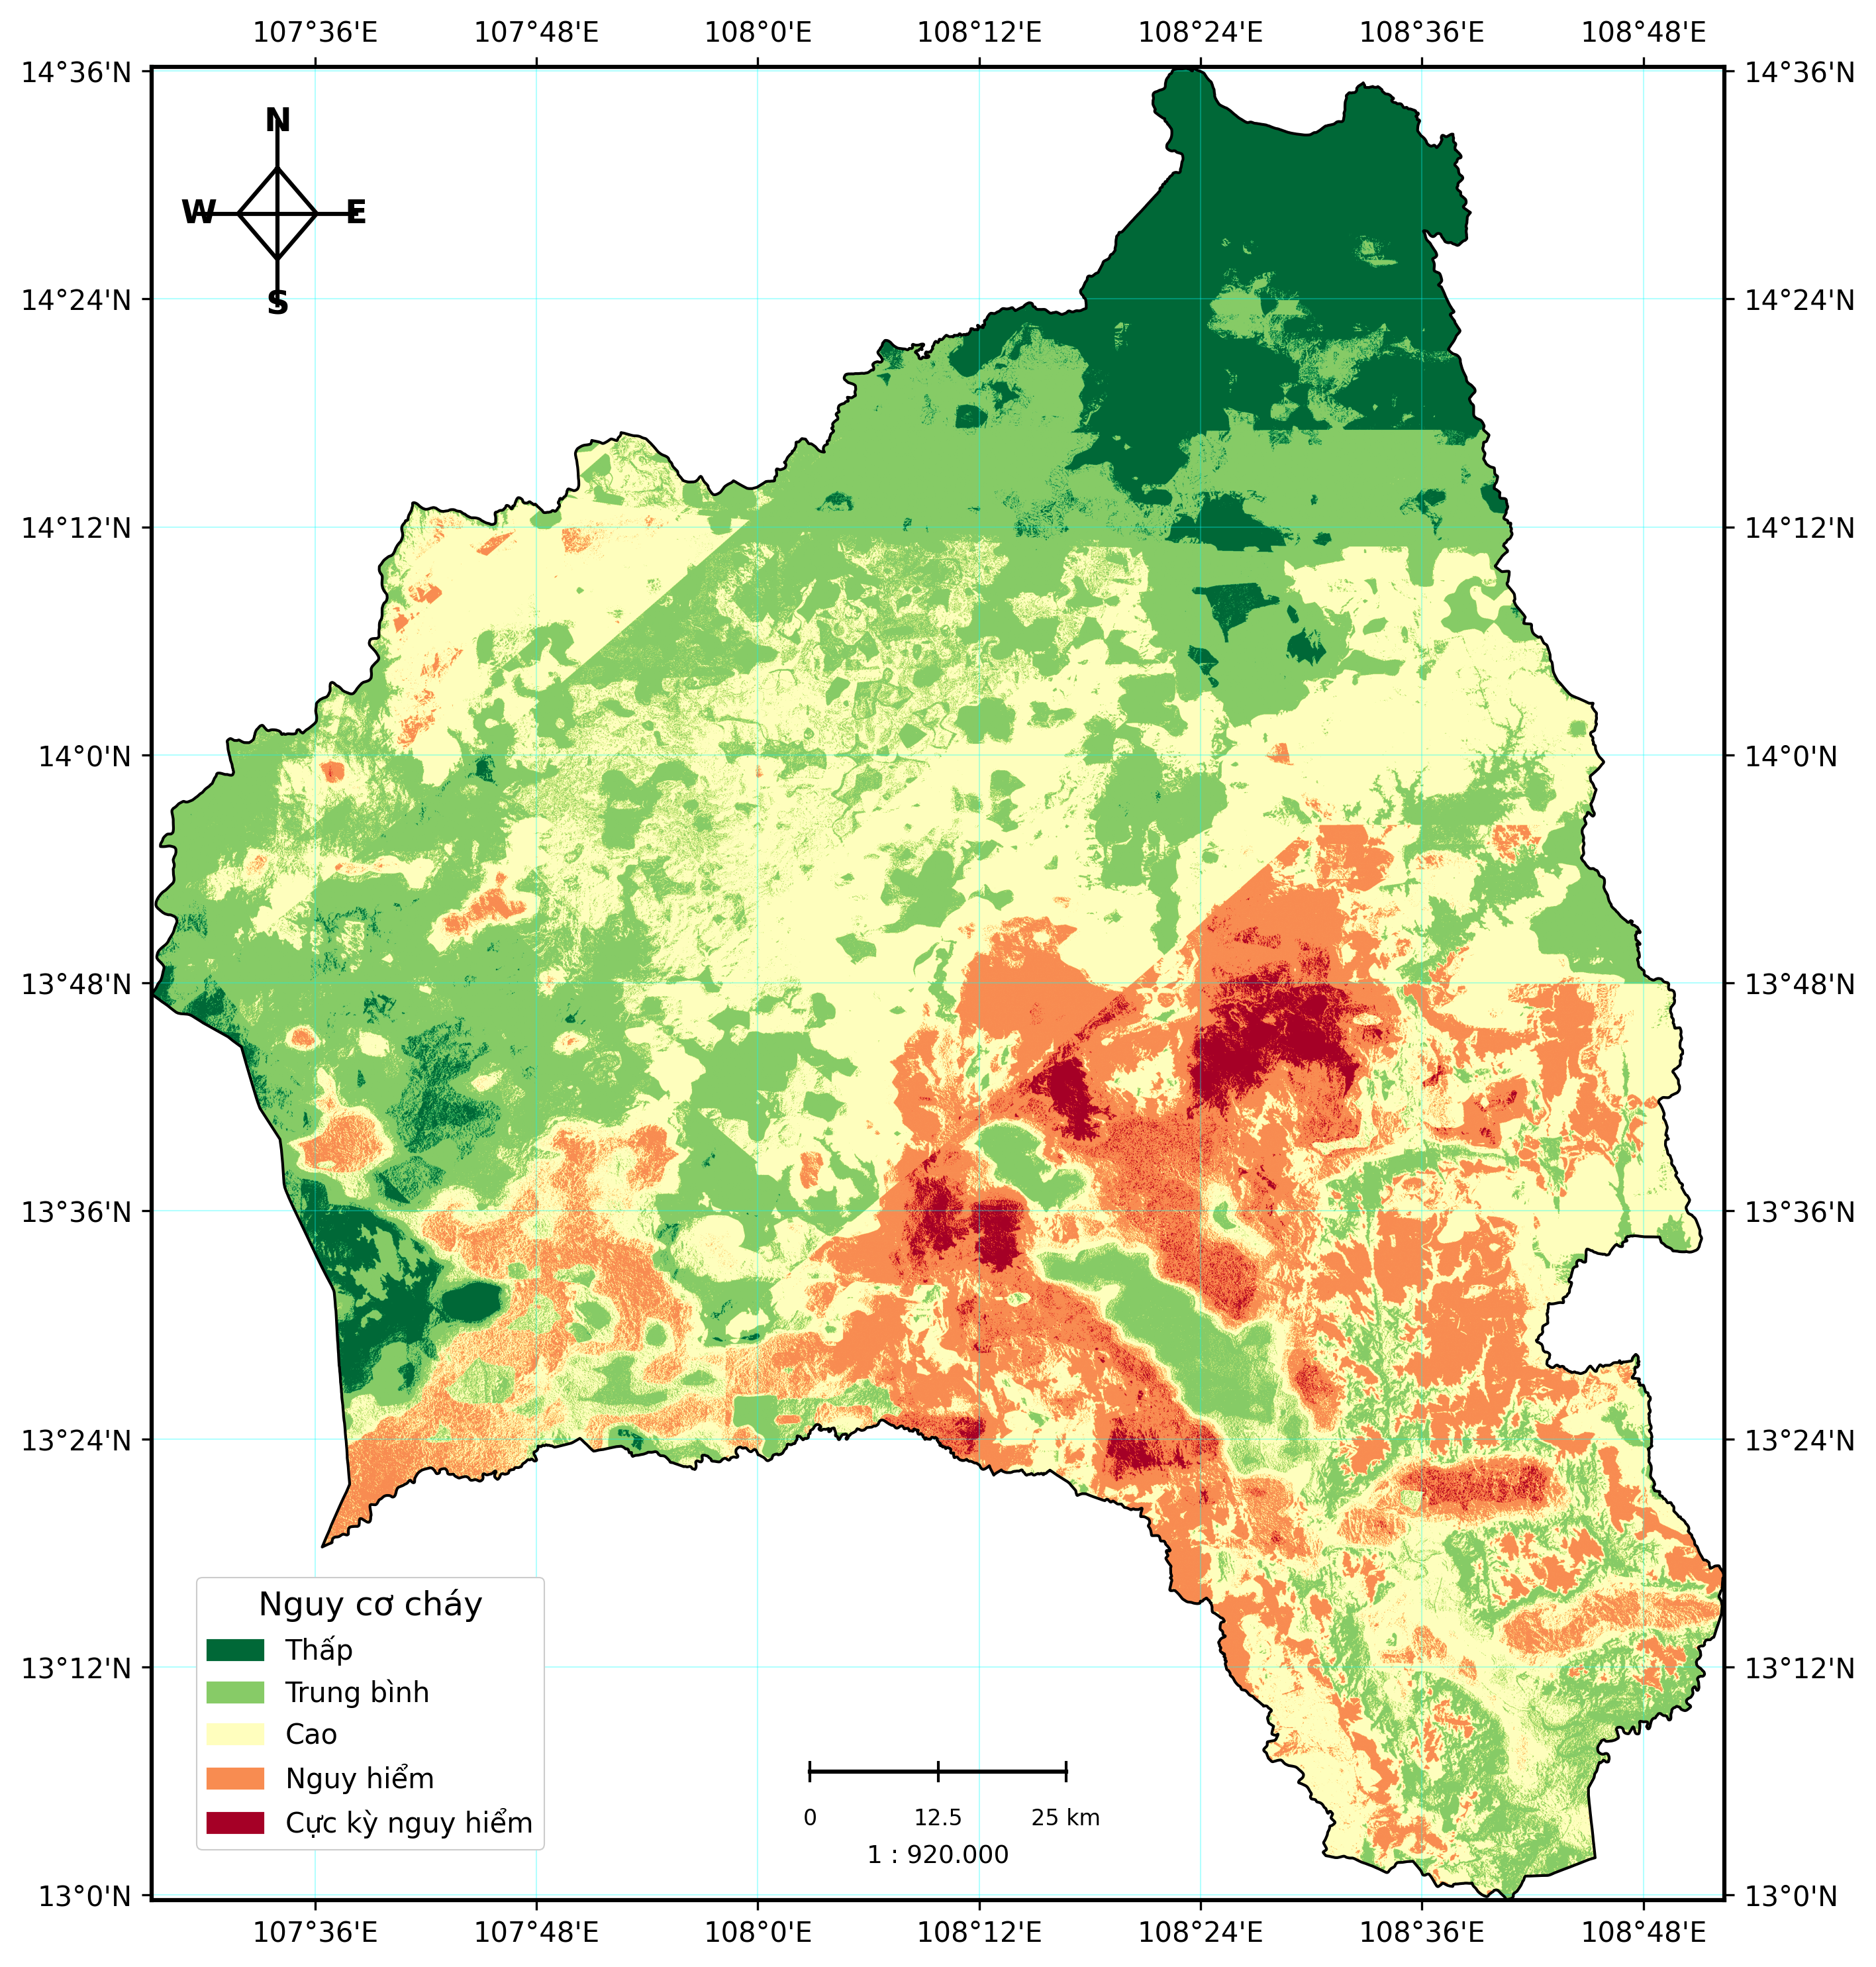
\includegraphics[width=1\textwidth]{GTB_Risk.png}
\caption{Bản đồ dự đoán nguy cơ cháy rừng tỉnh Gia Lai sử dụng mô hình Gradient Tree Boosting.}
\label{fig:ban_do_nguy_co_gtb}
\end{figure}

\subsection{Thống kê Diện tích theo Cấp độ Nguy cơ} % Mục con 4.3: Thống kê Diện tích (trước đây là 3.7)
Thống kê diện tích và tỷ lệ phần trăm của từng cấp độ nguy cơ cháy (dựa trên mô hình Random Forest và Gradient Tree Boosting) được trình bày trong Bảng~\ref{tab:thong_ke_dien_tich_nguy_co_rf} và Bảng~\ref{tab:thong_ke_dien_tich_nguy_co_gtb}.

% RF model
\begin{table}[H] % Bảng thống kê diện tích theo cấp độ nguy cơ cho RF
\centering
\caption{Thống kê diện tích và tỷ lệ phần trăm theo từng cấp độ nguy cơ cháy (Mô hình RF).}
\label{tab:thong_ke_dien_tich_nguy_co_rf}
\begin{tabular}{lcc}
\toprule
\textbf{Cấp độ nguy cơ} & \textbf{Diện tích (ha)} & \textbf{Tỷ lệ (\%)} \\ % Chú ý escape dấu % là \%
\midrule
1: Thấp & 75,830.850 & 4.9\% \\
2: Trung bình & 471,075.570 & 30.3\% \\
3: Cao & 867,867.390 & 55.8\% \\
4: Nguy hiểm & 192,581.460 & 12.4\% \\
5: Cực kỳ nguy hiểm & 823.320 & 0.1\% \\
\midrule
\textbf{Tổng cộng} & 1,608,178.590 & 100\% \\ % Tổng được tính lại
\bottomrule
\end{tabular}
\end{table}
\FloatBarrier

% GTB model
\begin{table}[H] % Bảng thống kê diện tích theo cấp độ nguy cơ cho GTB
\centering
\caption{Thống kê diện tích và tỷ lệ phần trăm theo từng cấp độ nguy cơ cháy (Mô hình GTB).}
\label{tab:thong_ke_dien_tich_nguy_co_gtb}
\begin{tabular}{lcc}
\toprule
\textbf{Cấp độ nguy cơ} & \textbf{Diện tích (ha)} & \textbf{Tỷ lệ (\%)} \\
\midrule
1: Thấp & 145,292.310 & 9.3\% \\
2: Trung bình & 535,017.060 & 34.4\% \\
3: Cao & 605,722.050 & 38.9\% \\
4: Nguy hiểm & 289,231.560 & 18.6\% \\
5: Cực kỳ nguy hiểm & 32,915.610 & 2.1\% \\
\midrule
\textbf{Tổng cộng} & 1,608,178.590 & 100\% \\ % Tổng được tính lại
\bottomrule
\end{tabular}
\end{table}
\FloatBarrier

\section{Thảo luận} % Bắt đầu Mục 5: Thảo luận
Nghiên cứu này đã thành công trong việc xây dựng và đánh giá các mô hình học máy để dự đoán nguy cơ cháy rừng tại tỉnh Gia Lai bằng cách sử dụng dữ liệu viễn thám đa nguồn trên nền tảng Google Earth Engine. Kết quả đánh giá trên tập kiểm tra cho thấy mô hình RF thể hiện hiệu suất vượt trội hơn trong việc xác định các khu vực có nguy cơ cháy, với độ chính xác tổng thể 93.05\% và F1-score cho lớp cháy 0.9317, cao hơn đáng kể so với mô hình GTB (83.81\% và 0.8412). Tuy nhiên, kết quả kiểm định chéo 5-fold trên tập huấn luyện cho thấy cả hai mô hình có độ chính xác trung bình khá tương đồng (RF: 77.90\%, GTB: 77.28%). Sự chênh lệch lớn giữa độ chính xác trên tập kiểm tra và độ chính xác từ kiểm định chéo của mô hình RF (93.05\% so với 77.90\%) so với mô hình GTB (83.81% so với 77.28%) cho thấy RF có thể đã học các đặc điểm của tập huấn luyện cụ thể tốt hơn, hay có khả năng overfitting nhiều hơn so với GTB, mặc dù GTB có hiệu suất tổng thể trên tập kiểm tra thấp hơn.

Phân tích độ quan trọng của các biến (dựa trên kết quả từ cả hai mô hình) đã chỉ ra rằng nhiệt độ bề mặt đất (Temperature), độ cao địa hình (DEM), lượng mưa (Precipitation) và tốc độ gió (WindSpeed) đóng vai trò quyết định trong việc hình thành nguy cơ cháy tại khu vực nghiên cứu. Đây là những yếu tố liên quan trực tiếp đến điều kiện khí hậu và địa hình, điều này phù hợp với lý thuyết về cơ chế hình thành cháy rừng. Điều đáng chú ý là các chỉ số thực vật truyền thống như NDVI không nằm trong top 5 biến quan trọng nhất đối với cả hai mô hình, mặc dù chúng thường được coi là chỉ báo quan trọng của trạng thái thực vật và nguy cơ cháy trong nhiều nghiên cứu khác. Ví dụ, đối với mô hình RF, 5 biến quan trọng nhất là Temperature, DEM, Precipitation, WindSpeed, và NBR; trong khi đối với GTB là Temperature, WindSpeed, Precipitation, DEM, và EVI.

Bản đồ nguy cơ cháy được tạo ra từ hai mô hình (Hình~\ref{fig:ban_do_nguy_co_rf} và~\ref{fig:ban_do_nguy_co_gtb}) cho thấy sự phân bố không gian của các vùng có mức độ rủi ro khác nhau. Nhìn chung, cả hai bản đồ đều xác định các khu vực có nguy cơ cao tập trung ở phía trung tâm và phía đông của tỉnh, tuy nhiên bản đồ từ mô hình RF có vẻ mịn hơn và ít phân mảnh hơn so với GTB. Điều này có thể giải thích do đặc tính khác nhau của hai thuật toán: RF xây dựng nhiều cây quyết định độc lập và lấy trung bình kết quả, trong khi GTB xây dựng các cây tuần tự để khắc phục lỗi của các cây trước đó.

Khi so sánh với bản đồ các điểm cháy thực tế (Hình~\ref{fig:diem_chay_thuc_te}), có thể thấy rằng phần lớn các điểm cháy ghi nhận được nằm trong những vùng được dự đoán có nguy cơ từ cao đến rất cao, đặc biệt là theo bản đồ từ mô hình RF. Điều này góp phần xác nhận tính hiệu quả của mô hình trong việc xác định các khu vực có nguy cơ cháy cao.

\section{Kết luận} % Bắt đầu Mục 6: Kết luận
Nghiên cứu này đã chứng minh tiềm năng của việc tích hợp dữ liệu viễn thám và các thuật toán học máy tiên tiến trên nền tảng Google Earth Engine để xây dựng bản đồ dự đoán nguy cơ cháy rừng hiệu quả cho tỉnh Gia Lai. Cả hai mô hình RF và GTB đều cho thấy hiệu suất tốt, với mô hình RF đạt độ chính xác tổng thể cao hơn (93.05\%) nhưng mô hình GTB có khả năng tổng quát hóa tốt hơn trên dữ liệu mới theo kết quả cross-validation.

Phân tích độ quan trọng của các biến đã xác định bốn yếu tố có ảnh hưởng lớn nhất đến nguy cơ cháy rừng tại Gia Lai, bao gồm: nhiệt độ bề mặt đất (Temperature), độ cao địa hình (DEM), lượng mưa (Precipitation) và tốc độ gió (WindSpeed). Việc sử dụng dữ liệu điểm cháy thực tế từ MODIS làm nhãn đánh giá đã đóng vai trò quan trọng trong việc đánh giá hiệu suất của mô hình. Kết quả này nhấn mạnh vai trò quan trọng của các yếu tố khí hậu và địa hình trong việc xác định nguy cơ cháy, và gợi ý rằng các nỗ lực giám sát cháy rừng nên tập trung đặc biệt vào những khu vực có nhiệt độ cao, độ cao trung bình, lượng mưa thấp và tốc độ gió mạnh.

Bản đồ nguy cơ cháy rừng được tạo ra từ mô hình RF là một công cụ có giá trị, có thể hỗ trợ đắc lực cho cơ quan quản lý rừng và phòng chống cháy rừng tại Gia Lai trong việc phân bổ nguồn lực, lập kế hoạch tuần tra và triển khai các biện pháp phòng ngừa hiệu quả, đặc biệt tại các khu vực có nguy cơ cao và cực kỳ nguy hiểm đã được xác định trên bản đồ.

Các hướng nghiên cứu tiếp theo có thể tập trung vào: (1) Tích hợp các yếu tố xã hội-kinh tế và hoạt động của con người vào mô hình dự báo; (2) Phát triển mô hình dự báo theo thời gian thực hoặc ngắn hạn để hỗ trợ cảnh báo sớm; (3) Khảo sát thực địa để kiểm chứng và hiệu chỉnh kết quả mô hình; và (4) Mở rộng phạm vi áp dụng cho các khu vực khác có nguy cơ cháy rừng cao ở Việt Nam.

\section{Đề xuất giải pháp}
\subsection{Giải pháp kỹ thuật}
\paragraph{Hệ thống giám sát thời gian thực:}
Thứ nhất, phát triển hệ thống tự động cập nhật dữ liệu vệ tinh hàng ngày. Thứ hai, tích hợp cảm biến IoT để đo các thông số môi trường tại chỗ. Thứ ba, xây dựng dashboard trực quan hóa dữ liệu theo thời gian thực.

\paragraph{Cải thiện mô hình dự báo:}
Đầu tiên, tích hợp thêm dữ liệu về hoạt động con người. Tiếp theo, phát triển mô hình dự báo ngắn hạn (3-5 ngày). Cuối cùng, tối ưu hóa độ phân giải không gian của bản đồ nguy cơ.

\subsection{Giải pháp quản lý}
\paragraph{Giải pháp ngắn hạn:}
Một là, tăng cường tuần tra tại các khu vực nguy cơ cao. Hai là, xây dựng đường băng cản lửa tại vị trí trọng yếu. Ba là, bố trí lực lượng ứng phó theo bản đồ nguy cơ.

\paragraph{Giải pháp dài hạn:}
Trước hết, quy hoạch lại cấu trúc rừng dựa trên bản đồ nguy cơ. Sau đó, đầu tư hệ thống quan trắc tự động. Cuối cùng, đào tạo nguồn nhân lực chuyên môn.

\subsection{Giải pháp cộng đồng}
\paragraph{Nâng cao nhận thức:}
Thứ nhất, tổ chức các buổi tập huấn cho người dân. Thứ hai, phát tờ rơi hướng dẫn phòng cháy. Thứ ba, xây dựng mạng lưới tình nguyện viên giám sát rừng.

\paragraph{Phối hợp đa bên:}
Đầu tiên, thiết lập cơ chế phối hợp giữa các bên liên quan. Tiếp theo, xây dựng quy trình báo cáo và xử lý sự cố. Sau cùng, tổ chức diễn tập phòng cháy định kỳ.
\section*{Lời cảm ơn} % Phần Lời cảm ơn
Nghiên cứu này được thực hiện với sự hỗ trợ của TS. Hà Minh Cường và ThS. Hoàng Tích Phúc của Viện Công nghệ Hàng không Vũ trụ, Trường Đại học Công nghệ - Đại học Quốc gia Hà Nội. Chúng tôi xin chân thành cảm ơn.

\section*{Mã nguồn và Dữ liệu} % Phần Mã nguồn và Dữ liệu trên GitHub
Các bộ dữ liệu gốc được sử dụng trong nghiên cứu này có nguồn gốc từ các kho lưu trữ công cộng đã được mô tả chi tiết trong phần Phương pháp. Toàn bộ mã nguồn xử lý dữ liệu, huấn luyện mô hình và tạo ra các kết quả được trình bày trong bài báo này được công bố công khai tại GitHub: {\color{blue}\url{https://github.com/Luongoc-1307/forest-firet}}. Các sản phẩm trung gian, bao gồm dữ liệu đã xử lý và bản đồ nguy cơ chi tiết, sẵn sàng được cung cấp theo yêu cầu hợp lý gửi đến tác giả liên hệ, nhằm mục đích hỗ trợ việc kiểm tra và tái tạo kết quả nghiên cứu.


\printbibliography % In danh mục tài liệu tham khảo

\end{document} % Kết thúc tài liệu